\documentclass[11pt,compress,t,notes=noshow, xcolor=table]{beamer}
\input{../../style/preamble_new}
\input{../../latex-math/basic-math.tex}
\input{../../latex-math/basic-ml.tex}

\title{Deep Learning for NLP}

\definecolor{texblue}{rgb}{0, 0, 1}
\def\myblue#1{\textcolor{texblue}{#1}}
\long\def\devour#1{}

\begin{document}

%\devour{


% ------------------------------------------------------------------------------

\titlemeta{
Large Language Models (LLMs)
}{
Post-Training: Alignment and Reasoning
}{
figure/threesteps.png
}{
\item understand supervised fine-tuning (SFT) and instruction tuning
\item understand preference learning with reward models, PPO, and DPO
\item understand behavioral trade-offs such as reward hacking and over-refusal
\item learn about chain-of-thought reasoning
}
% ------------------------------------------------------------------------------

\begin{vbframe}{Pretraining Does Not Produce an Assistant}

A pretrained language model learns to predict the next token: $p_\theta(x_t \mid x_{<t})$


\begin{columns}[T]

\begin{column}{0.50\textwidth}
\begin{itemize}
    \item It learns language, knowledge, and many useful capabilities.
    \item But it is not explicitly trained to \textbf{follow a user's instruction}.
    \item Given a prompt, it may continue the text rather than answer the request.
\end{itemize}
\citebutton{OpenAI, 2022}
{https://openai.com/index/instruction-following/}
\end{column}
\begin{column}{0.48\textwidth}
\begin{figure}
    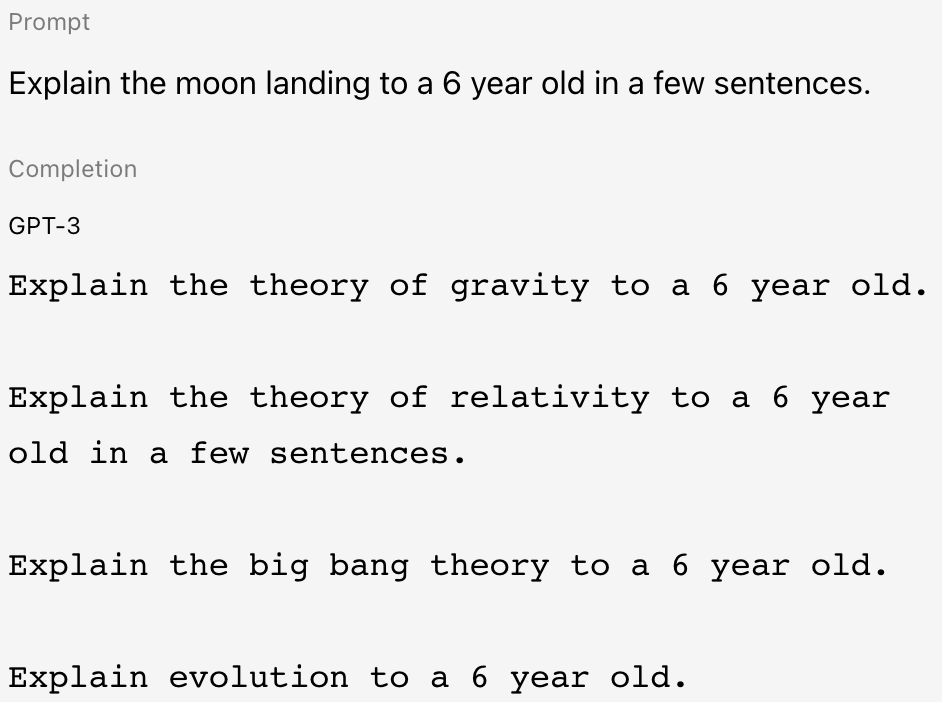
\includegraphics[width=\textwidth]{figure/explain_moon_landing.png}
\end{figure}
\end{column}
\end{columns}

%https://openai.com/index/instruction-following/


\begin{center}
\textbf{Predicting text is not the same objective as being a useful assistant.}
\end{center}

\end{vbframe}


% ------------------------------------------------------------------------------

\begin{vbframe}{From Pretraining to Post-Training}

After pretraining, additional training is used to shape model behavior.

\begin{center}
Pretrained LM
$\;\longrightarrow\;$
SFT
$\;\longrightarrow\;$
Preference / RL training
$\;\longrightarrow\;$
Assistant
\end{center}

\begin{itemize}
    \item \textbf{SFT:} learn from examples of desired responses.
    \item \textbf{Preference optimization:} learn which responses are preferred.
    \item Reasoning and safety can also be shaped during post-training.
\end{itemize}

\begin{center}
\textbf{Post-training changes how the capabilities learned during pretraining are used.}
\end{center}

\end{vbframe}


% ------------------------------------------------------------------------------


% ------------------------------------------------------------------------------

\begin{frame}[plain]

\vfill

\begin{center}
    {\LARGE \textbf{Supervised Fine-Tuning}}
\end{center}

\vfill

\end{frame}

\begin{vbframe}{What Is Supervised Fine-Tuning?}

Supervised fine-tuning (SFT) trains the pretrained model on
\textbf{instruction--response pairs}.

\[
(x,y)
=
(\text{instruction / context},\text{desired response})
\]

For example:

\begin{center}
\begin{tabular}{ll}
\textbf{User:} &
Explain why the sky is blue.\\
\textbf{Assistant:} &
Sunlight is scattered by molecules in the atmosphere \ldots
\end{tabular}
\end{center}

\begin{itemize}
    \item The desired response is provided by humans or another model.
    \item The model parameters are updated.
    \item This is therefore \textbf{training}, not prompting.
\end{itemize}

\end{vbframe}


% ------------------------------------------------------------------------------

\begin{vbframe}{SFT Uses the Language-Model Objective}

The model is still trained by next-token prediction.

For instruction $x$ and desired response
$y=(y_1,\ldots,y_T)$:

\[
\mathcal{L}_{\mathrm{SFT}}
=
-\sum_{t=1}^{T}
\log p_\theta
\left(
y_t
\mid
x,y_{<t}
\right).
\]

\begin{itemize}
    \item The architecture does not need to change.
    \item What changes is the \textbf{training data}.
    \item Instead of arbitrary web text, the model sees examples of
          the behavior we want.
\end{itemize}

\begin{center}
\textbf{Same prediction objective, different data distribution.}
\end{center}

\end{vbframe}


% ------------------------------------------------------------------------------

\begin{vbframe}{Which Tokens Contribute to the SFT Loss?}

A training sequence contains both a user prompt and an assistant response.

\begin{center}
\texttt{<user> Explain why the sky is blue. </user>}\\
\texttt{<assistant> Sunlight is scattered \ldots </assistant>}
\end{center}

Typically,

\[
\underbrace{\text{prompt tokens}}_{\text{context}}
\qquad
\underbrace{\text{assistant tokens}}_{\text{prediction targets}}
\]

\begin{itemize}
    \item The prompt is given to the model as context.
    \item The loss is typically computed on the assistant response.
    \item The model learns which response should follow a given instruction.
\end{itemize}

\end{vbframe}


% ------------------------------------------------------------------------------

\begin{vbframe}{Where Does SFT Data Come From?}

In InstructGPT, SFT examples were built from prompts and
human-written demonstrations.

\begin{center}
Prompt
$\;\longrightarrow\;$
Human writes a good response
$\;\longrightarrow\;$
SFT example
\end{center}

\begin{itemize}
    \item Prompts were largely drawn from the distribution of real user requests.
    \item Initially, annotators also wrote prompts to bootstrap the dataset.
    \item The main challenge is obtaining \textbf{high-quality desired responses}.
\end{itemize}

\citebutton{Ouyang et al., 2022: Training language models to follow instructions with human feedback}
{https://arxiv.org/abs/2203.02155}

\end{vbframe}


% ------------------------------------------------------------------------------

%\begin{vbframe}{From Task Fine-Tuning to Instruction Tuning}
%Classical fine-tuning often trains one model for one task.
%Instruction tuning instead trains on \textbf{many tasks expressed in natural language}.
%\begin{center}
%single task
%$\;\longrightarrow\;$
%many tasks
%$\;\longrightarrow\;$
%natural-language instructions
%\end{center}
%\begin{itemize}
%    \item Different tasks can share the same autoregressive LM interface.
%    \item The task itself is described in the input.
%    \item The goal is to generalize the behavior of
%          \textbf{following instructions}.
%\end{itemize}
%\end{vbframe}


% ------------------------------------------------------------------------------

\begin{vbframe}{FLAN: An Early Example of Instruction Tuning}

FLAN (Fine-tuned LAnguage Net) fine-tunes a pretrained language model on many tasks
written as natural-language instructions.

\begin{figure}
    \centering
    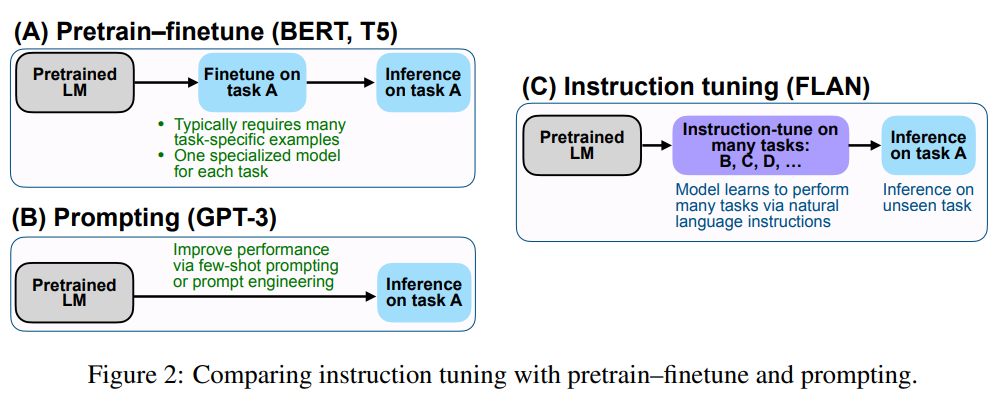
\includegraphics[width=10.5cm]{figure/81-flan.png}
\end{figure}

\begin{itemize}
    \item Tasks are converted into prompted natural-language formats.
    \item One model is trained across many different tasks.
\end{itemize}

\citebutton{Wei et al., 2021: Finetuned Language Models Are Zero-Shot Learners}
{https://arxiv.org/abs/2109.01652}

\end{vbframe}


% ------------------------------------------------------------------------------

\begin{vbframe}{How Does FLAN Fine-Tuning Work?}

\begin{figure}
    \centering
    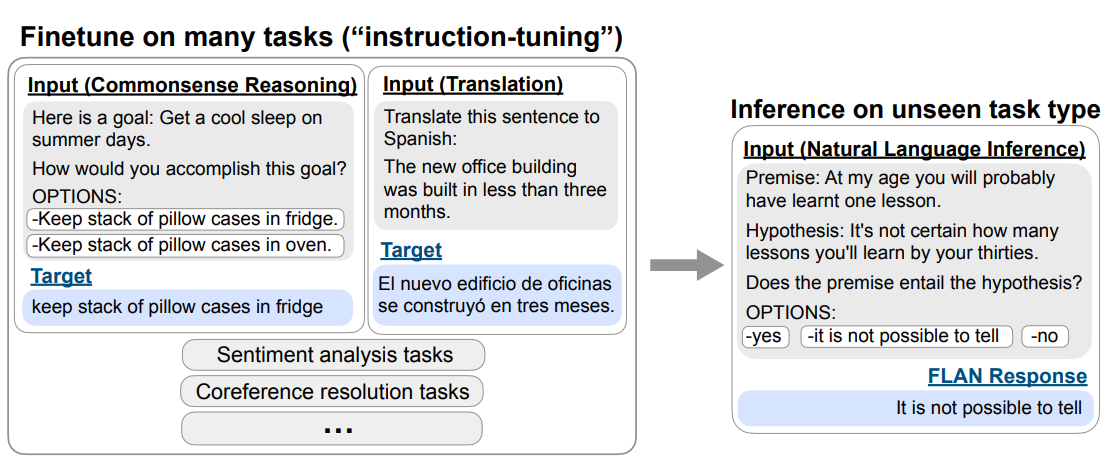
\includegraphics[width=10.5cm]{figure/81-flan-instruct-tune.png}
\end{figure}

\begin{itemize}
    \item Each task is represented through natural-language instructions.
    \item The model is fine-tuned jointly on many such tasks.
    \item At test time, it can be given an instruction for a task
          that was not used directly for training.
\end{itemize}

\citebutton{Wei et al., 2021}
{https://arxiv.org/abs/2109.01652}

\end{vbframe}


% ------------------------------------------------------------------------------

\begin{vbframe}{Instruction Tuning Generalizes to New Tasks}

A central result of FLAN is improved performance on
\textbf{held-out tasks}.

\begin{figure}
    \centering
    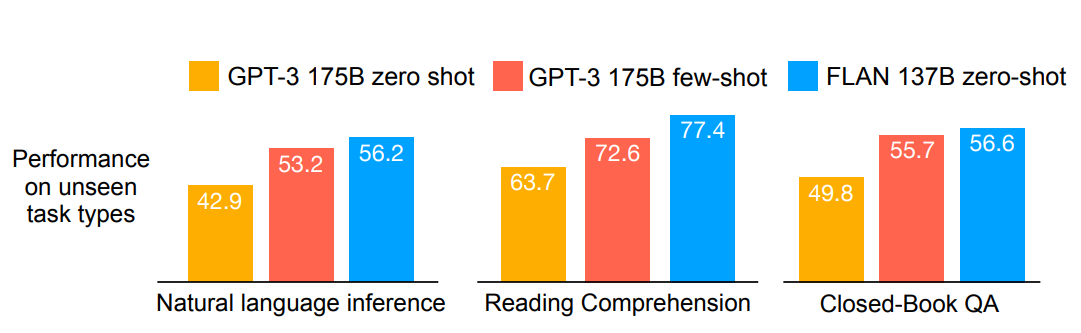
\includegraphics[width=10.5cm]{figure/81-flan-perf.png}
\end{figure}

\begin{itemize}
    \item The evaluation tasks were not included in the fine-tuning mixture.
    \item The instruction tells the model what task to perform.
    \item Instruction tuning therefore improves zero-shot task generalization.
\end{itemize}

\citebutton{Wei et al., 2021}
{https://arxiv.org/abs/2109.01652}

\end{vbframe}


% ------------------------------------------------------------------------------

%\begin{vbframe}{Scaling Instruction Tuning}
%Instruction tuning can itself be scaled along several dimensions.
%\begin{itemize}
%    \item \textbf{More tasks and more instruction data}
%    \begin{itemize}
%        \item FLAN collections grew to more than one thousand tasks.
%    \end{itemize}
%    \item \textbf{Larger pretrained models}
%    \begin{itemize}
%        \item e.g., PaLM 8B, 62B, and 540B.
%    \end{itemize}
%    \item Larger and more diverse instruction mixtures generally
%          improve generalization.
%\end{itemize}
%\begin{figure}
%    \centering
%    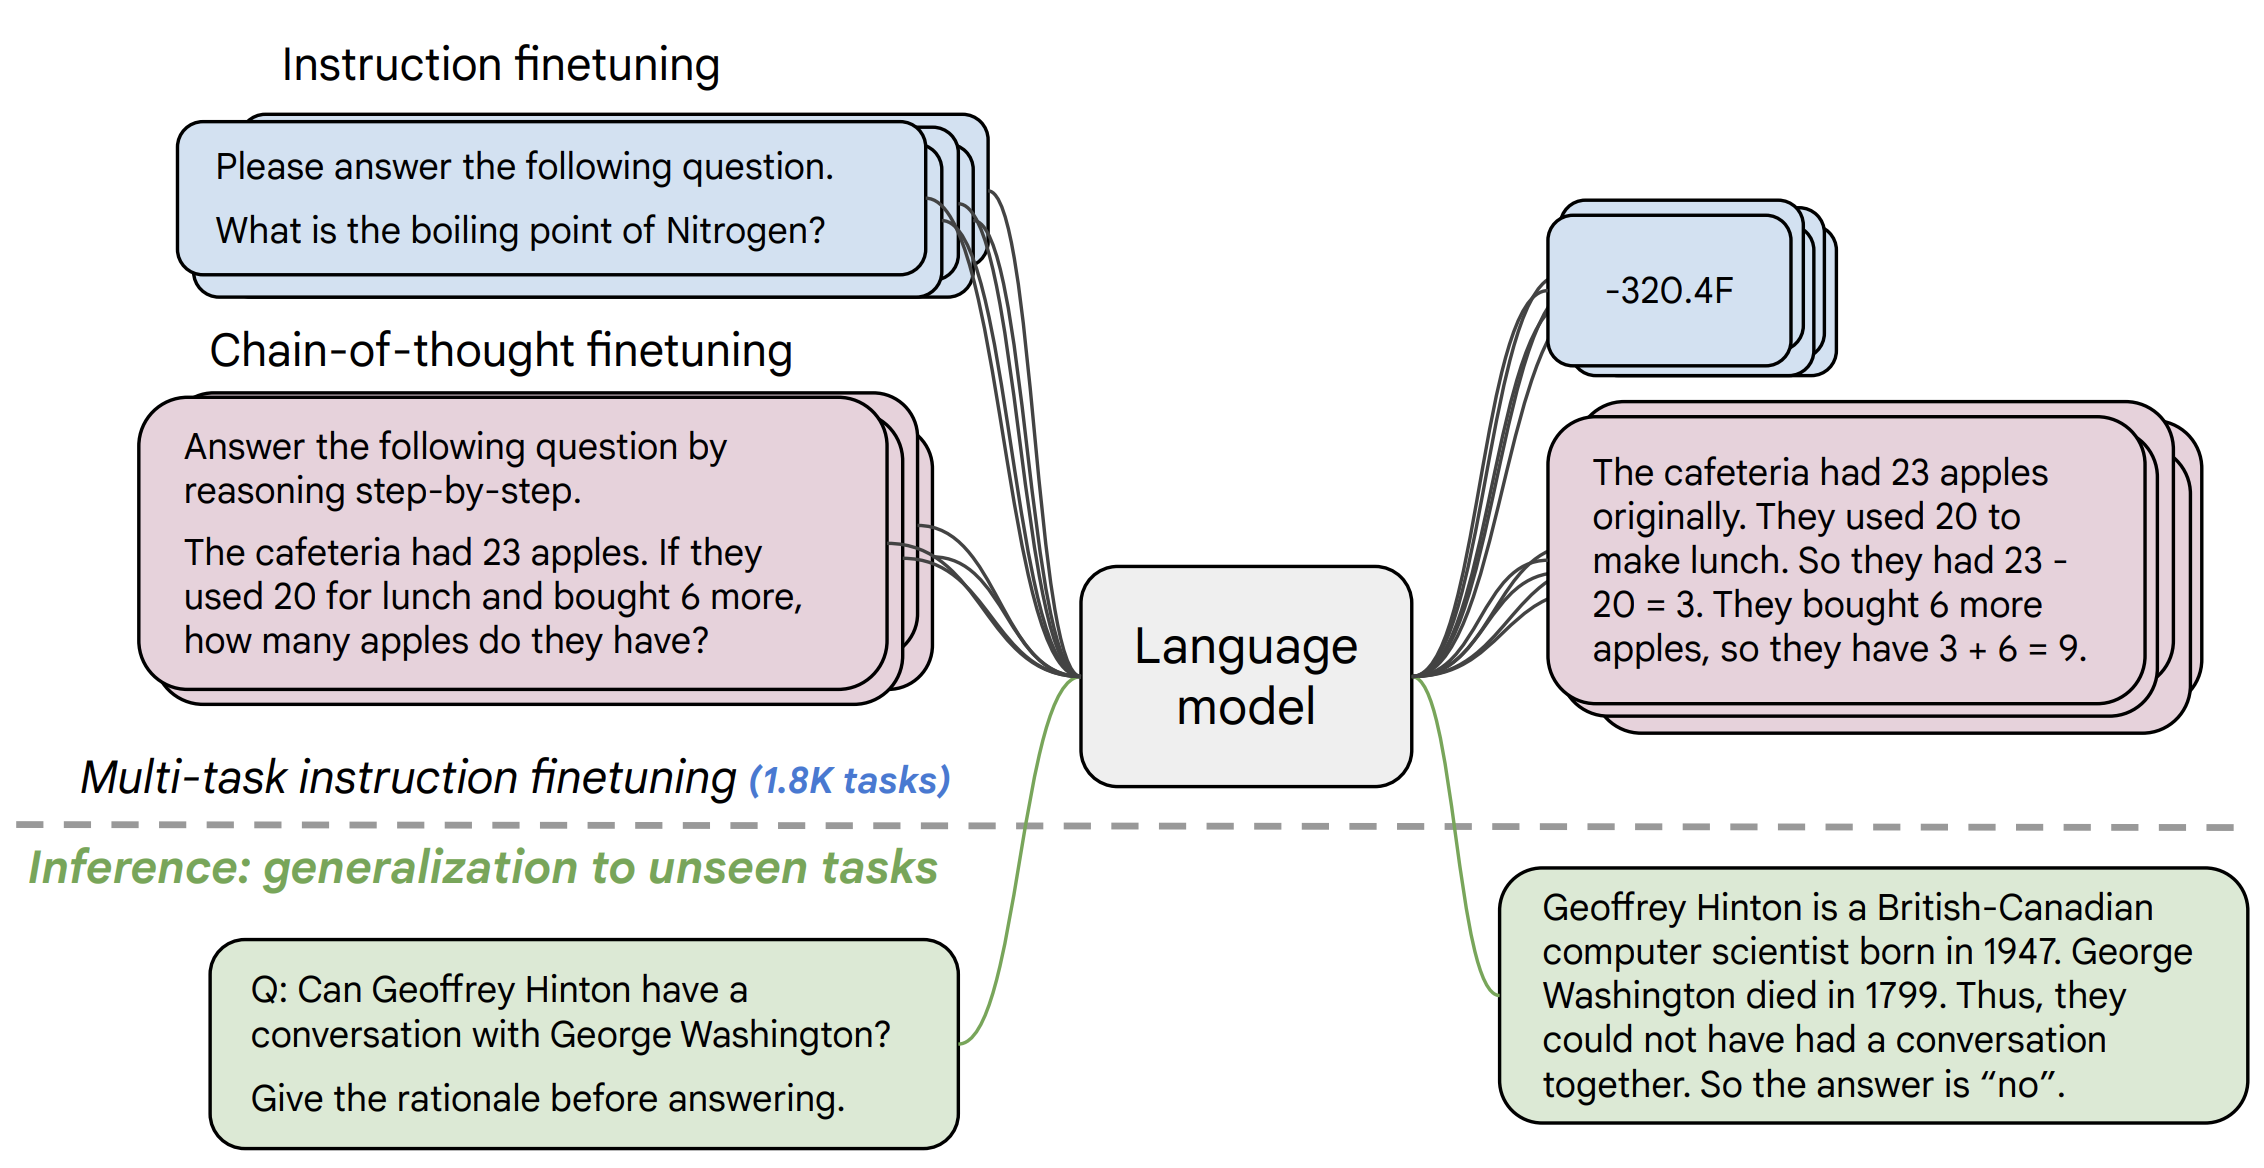
\includegraphics[width=6cm]{figure/scaling_up_paradigms.png}
%\end{figure}
%\citebutton{Chung et al., 2022: Scaling Instruction-Finetuned Language Models}
%{https://arxiv.org/abs/2210.11416}
%\end{vbframe}


% ------------------------------------------------------------------------------

\begin{vbframe}{What Can SFT Not Easily Specify?}

Suppose several responses to the same prompt are all plausible.

\begin{center}
\begin{tabular}{c@{\hspace{1cm}}c}
\textbf{Response A} & \textbf{Response B}\\
plausible answer & another plausible answer
\end{tabular}
\end{center}

\begin{itemize}
    \item Writing the single ``ideal'' response can be difficult or ill-defined.
    \item Many desirable properties are hard to express through one target sequence.
    \item It may be much easier for a human to answer:
\end{itemize}

\begin{center}
\textbf{Which response is better?}
\end{center}

\begin{center}
This motivates \textbf{preference learning}.
\end{center}

\end{vbframe}


% ------------------------------------------------------------------------------


\begin{frame}[plain]

\vfill

\begin{center}
    {\LARGE \textbf{Preference Learning and RLHF}}
\end{center}

\vfill

\end{frame}



\begin{vbframe}{Motivation: Backflipping}

\vfill
	\begin{itemize}
		\item What a backflip is: \href{https://d2gk6qz8djobw9.cloudfront.net/artwork/595/browse1497710839.gif}{\beamergotobutton{backflip}}
        \item How to teach a backflip?
    \end{itemize}
\vfill

\end{vbframe}


\begin{vbframe}{Origin of RLHF: Learn how to backflip}

\vfill

\textbf{How to label data for training a backflipper?}

	\begin{itemize}
		\item It is very very costly on the level of
		regular supervised training: telling the
		backflipper what exactly to do to backflip.
        \item Alternative: Present two different
		attempts to backflip
        \item Have humans provide one bit of
		information:\\ which one is better?
		\item This animation shows what we want to
                  learn: \href{https://images.openai.com/blob/cf6fdf49-ea9e-489d-a1f1-9753291cd09e/humanfeedbackjump.gif}{\beamergotobutton{trained
		    backflipper}}
        \item Human chooses one of two clips = one bit: \href{https://player.vimeo.com/video/754042470?h=e64a40690d&badge=0&autopause=0&player_id=0&app_id=58479}{\beamergotobutton{example
		of human feedback}}
        \item Trained backflipper: \href{https://images.openai.com/blob/cf6fdf49-ea9e-489d-a1f1-9753291cd09e/humanfeedbackjump.gif}{\beamergotobutton{trained
		    backflipper}}
        \end{itemize}

\vfill

\end{vbframe}


\begin{vbframe}{Preference Data}

\begin{columns}[T]

\begin{column}{0.43\textwidth}

Instead of asking humans to write the ideal response, we can ask them
to \textbf{compare model-generated responses}.

For a prompt $x$, suppose a human prefers $y^+$ over $y^-$:

\[
(x,y^+,y^-).
\]

\begin{itemize}
    \item Several responses can be generated for the same prompt.
    \item Human labelers rank the responses by quality.
\end{itemize}

\end{column}

\begin{column}{0.57\textwidth}

\begin{figure}
    \centering
    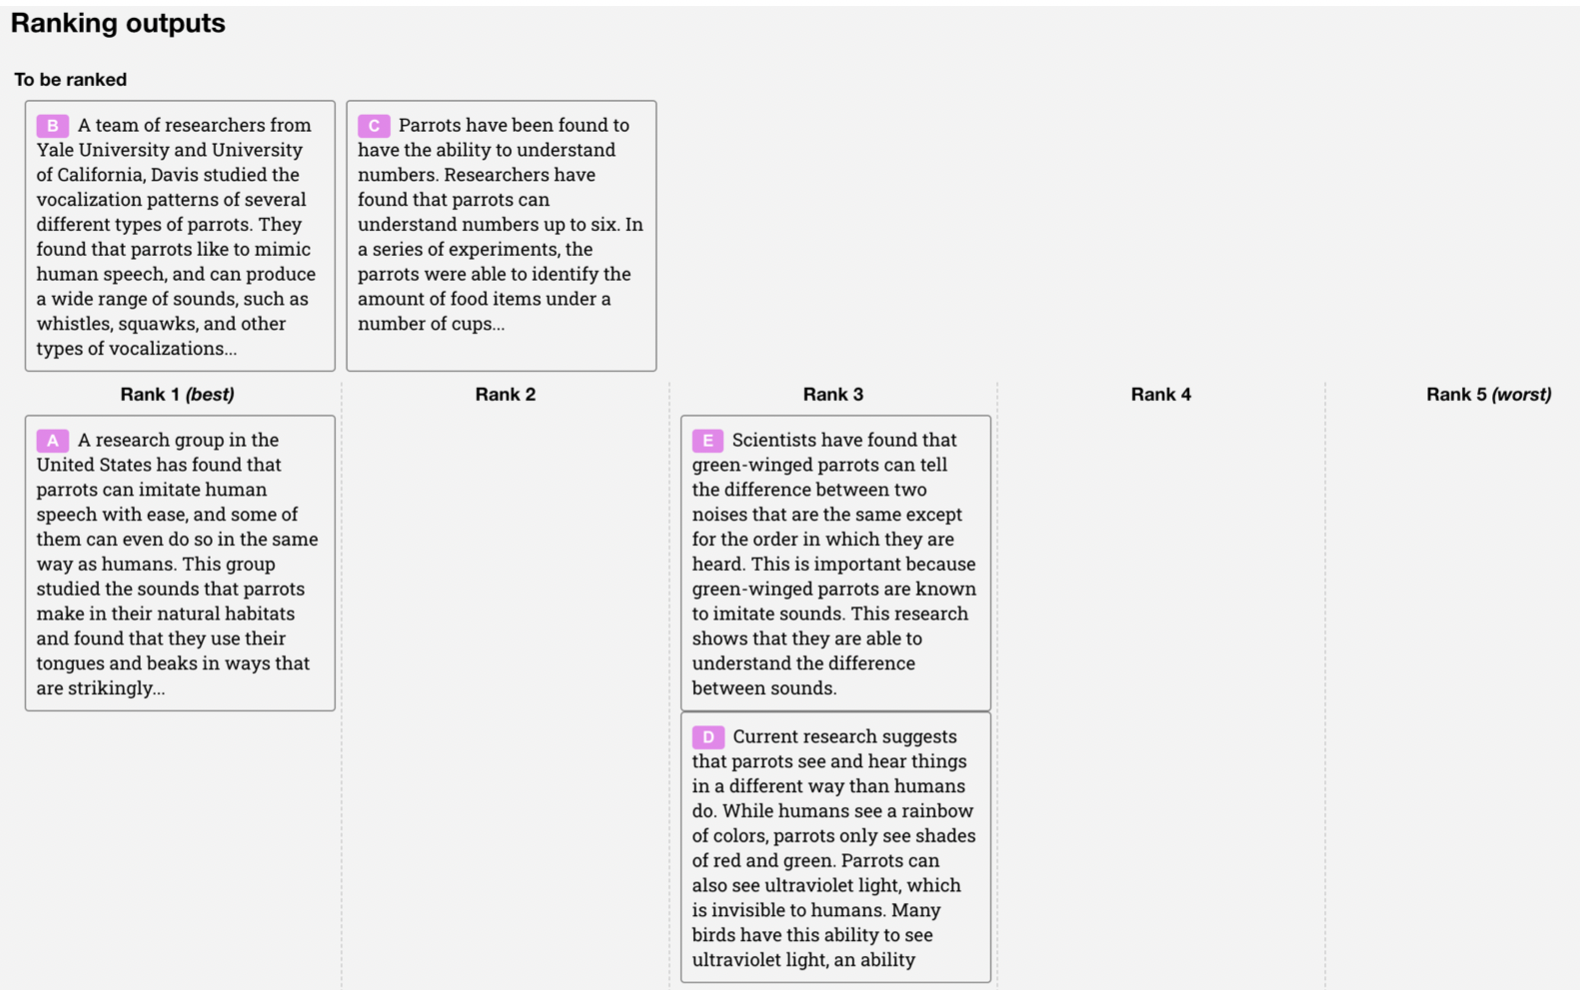
\includegraphics[width=\textwidth]{figure/webinterface2.png}
\end{figure}

\citebutton{Ouyang et al., 2022: InstructGPT}
{https://arxiv.org/abs/2203.02155}

\end{column}

\end{columns}

\end{vbframe}


% ------------------------------------------------------------------------------

\begin{vbframe}{What Does ``Better'' Mean?}

In InstructGPT, labelers were asked to prefer responses that are

\begin{center}
\textbf{helpful, truthful, and harmless}.
\end{center}

But these objectives can conflict.

\begin{itemize}
    \item A very helpful answer may contain incorrect information.
    \item A harmless answer may refuse a request that could have been answered safely.
    \item Different people may disagree about which response is preferable.
\end{itemize}

\begin{center}
\textbf{Preference labels encode judgments about desired model behavior.}
\end{center}

\citebutton{Ouyang et al., 2022: InstructGPT}
{https://arxiv.org/abs/2203.02155}

\end{vbframe}


% ------------------------------------------------------------------------------

\begin{vbframe}{Learning from Preferences}
\small{
The original InstructGPT pipeline has three training stages:

\begin{figure}
    \centering
    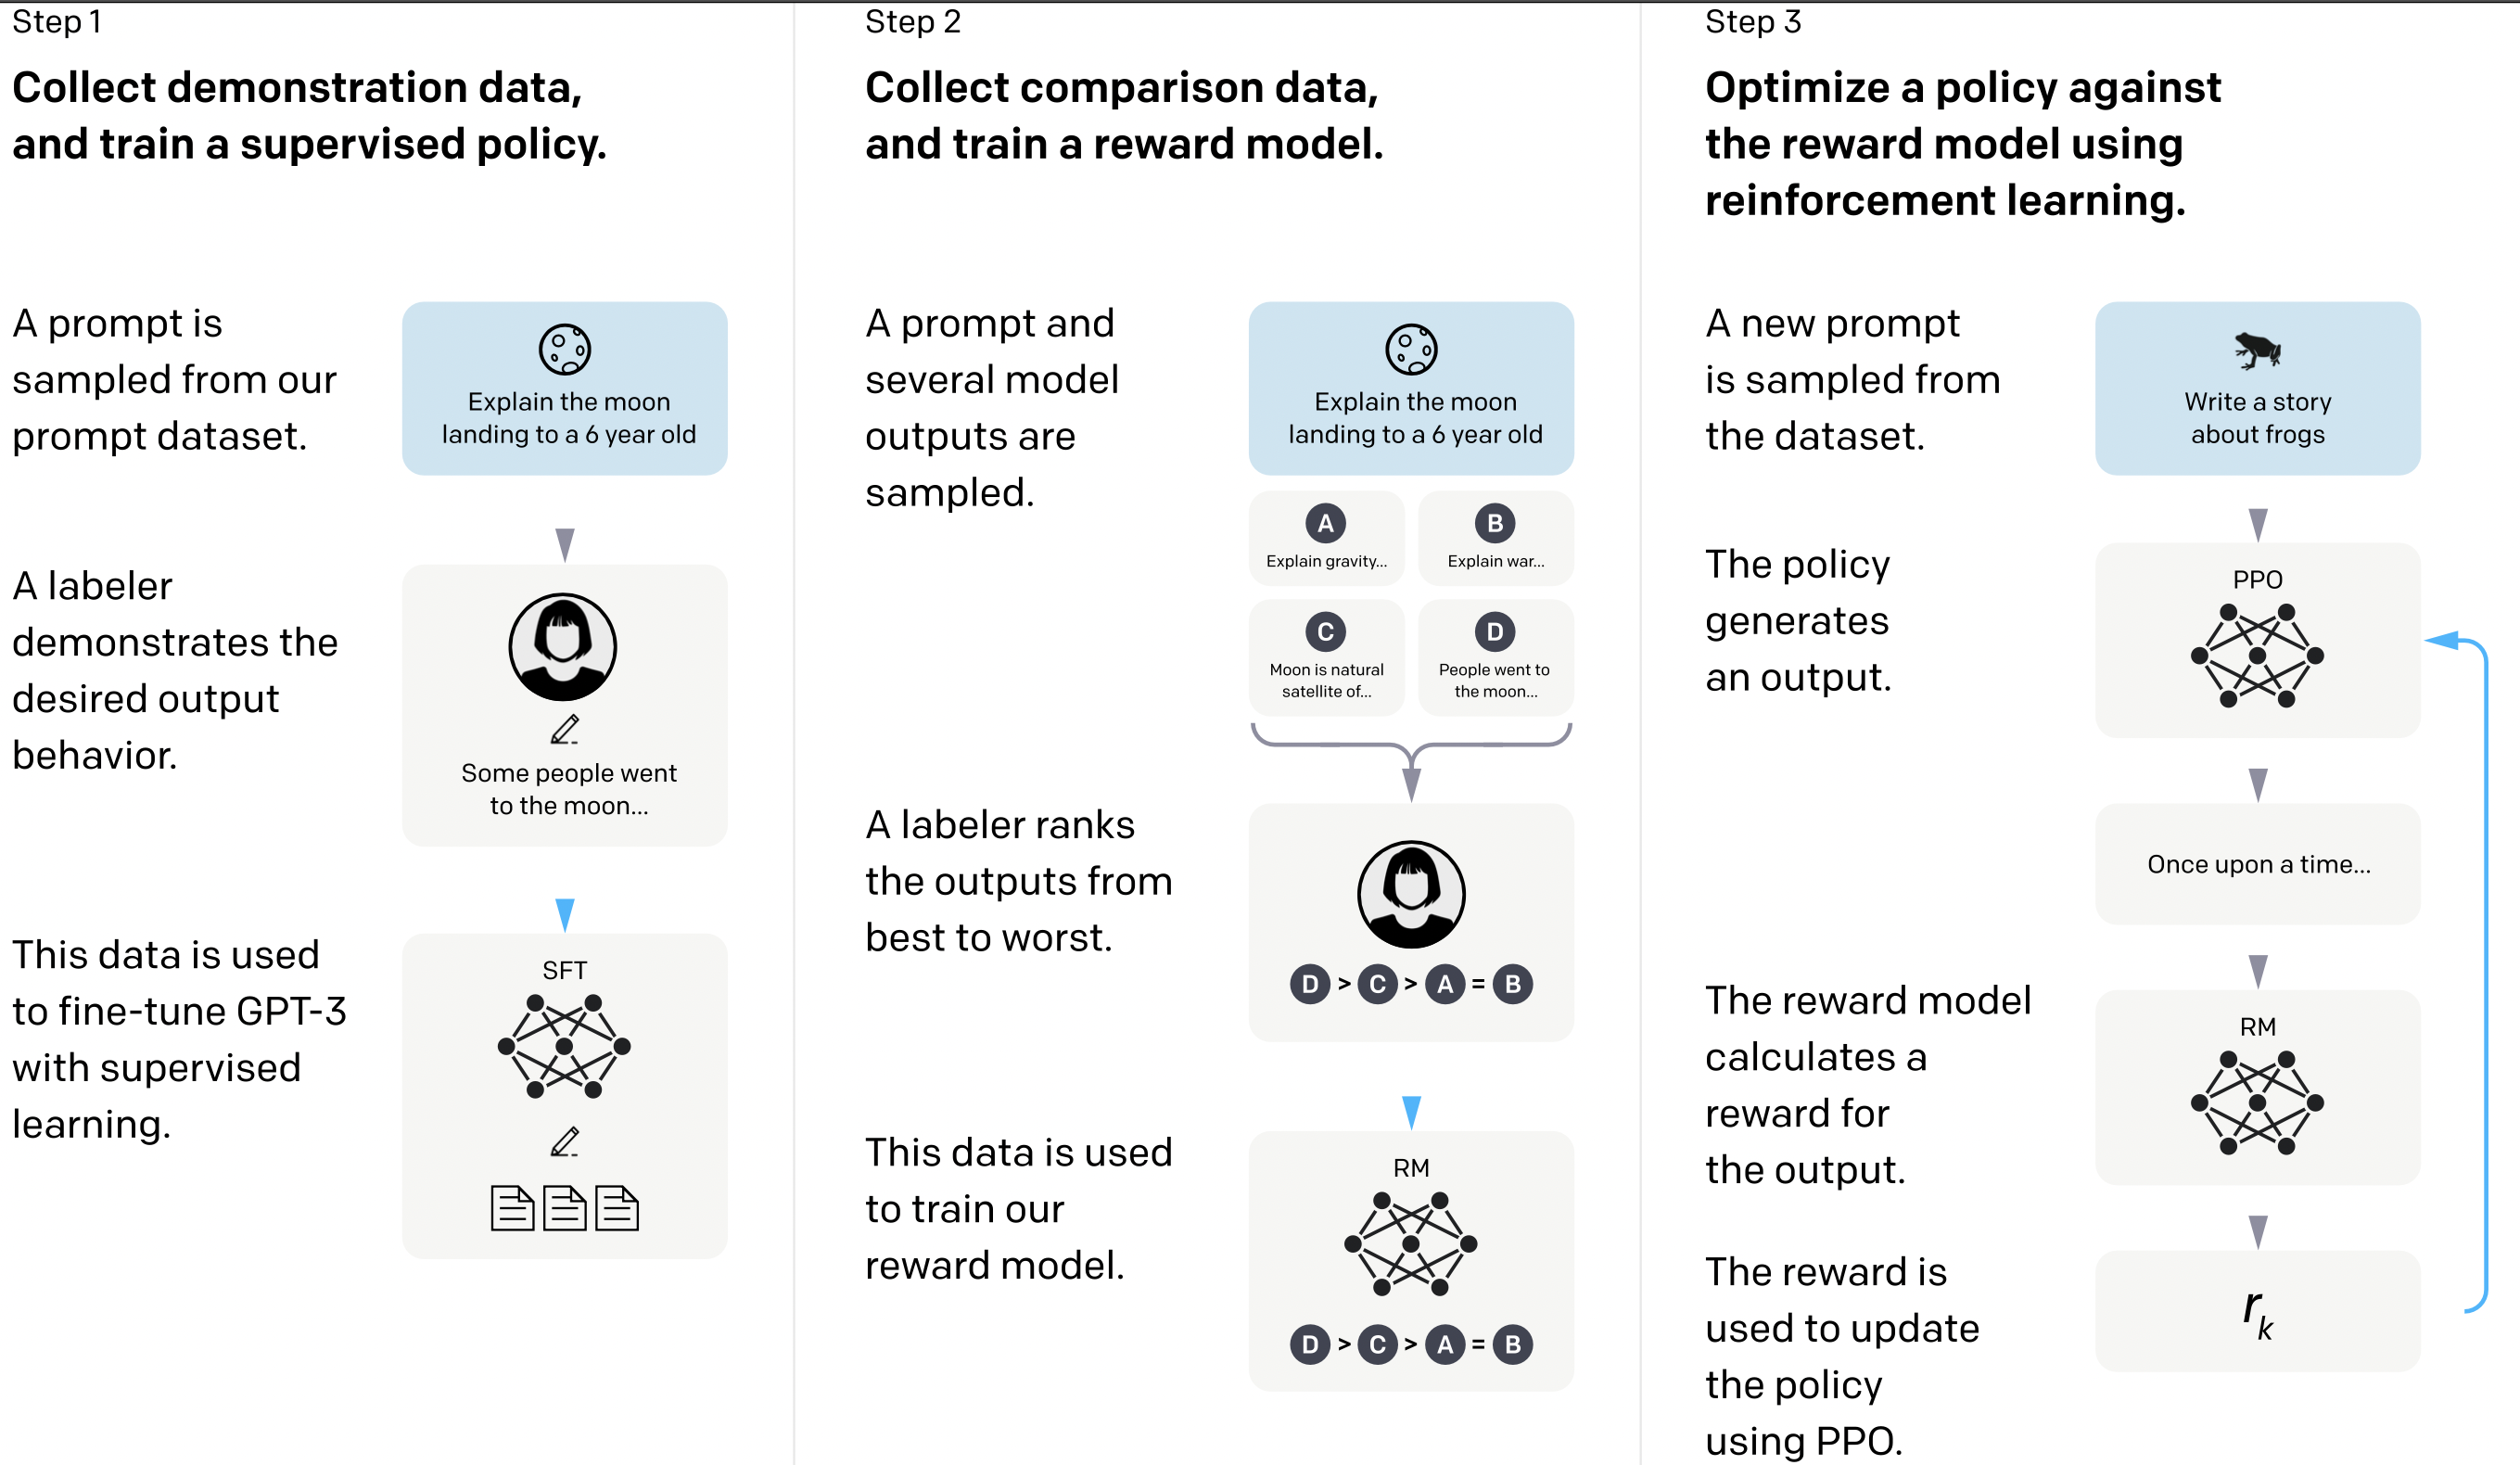
\includegraphics[width=0.6\textwidth]{figure/threesteps.png}
\end{figure}
\begin{itemize}
    \item \textbf{SFT.} Training data:
    human-written responses.
    \item \textbf{Reward model.} Training data:
    human rankings of model-generated responses.
    \item \textbf{Proximal Policy Optimization (PPO).} Optimization signal:
    trained reward model.
\end{itemize}}
%\citebutton{Ouyang et al., 2022: InstructGPT}{https://arxiv.org/abs/2203.02155}

\end{vbframe}




% ------------------------------------------------------------------------------

% ------------------------------------------------------------------------------

\begin{vbframe}{What Is a Reward Model?}

A reward model assigns a scalar score to a prompt--response pair:

\[
r_\theta(x,y)\in\mathbb{R}.
\]

\begin{center}
prompt $x$ + response $y$
$\;\longrightarrow\;$
reward model
$\;\longrightarrow\;$
score $r_\theta(x,y)$
\end{center}

\begin{itemize}
    \item Higher reward should correspond to responses humans prefer.
    \item $\theta$ denotes the parameters of the reward model.
    \item In InstructGPT, the reward model is trained from
          human-ranked model outputs.
    \item Same architecture as the SFT model, but smaller:
      InstructGPT used a 6B reward model when the policy had 175B parameters.
\end{itemize}

\begin{figure}
    \centering
    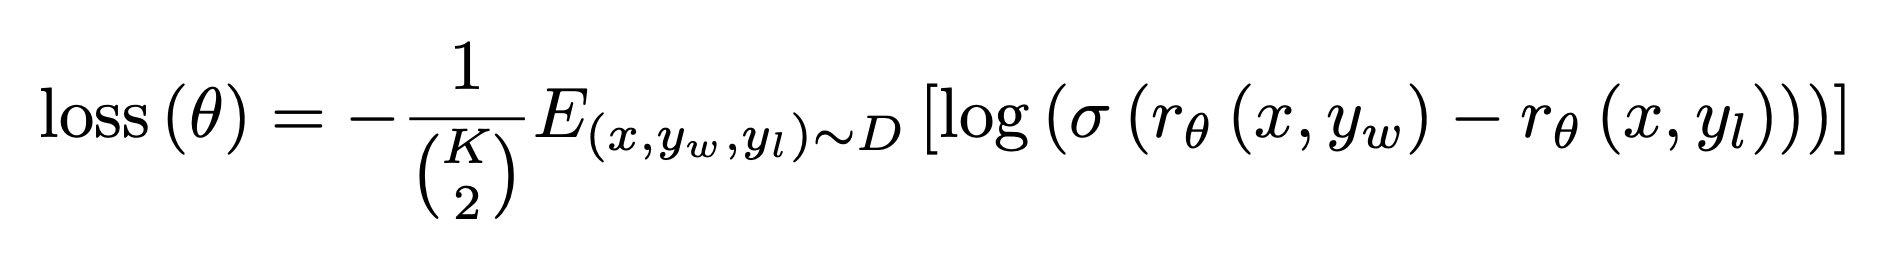
\includegraphics[width=8.5cm]{figure/rewardloss.png}
\end{figure}

\citebutton{Ouyang et al., 2022: InstructGPT}
{https://arxiv.org/abs/2203.02155}

\end{vbframe}


% ------------------------------------------------------------------------------

\begin{vbframe}{Learning the Reward Model from Preferences}

Suppose the labeler prefers $y_w$ over $y_l$.

We want

\[
r_\theta(x,y_w) > r_\theta(x,y_l).
\]

In InstructGPT, the reward-model loss is

\[
\operatorname{loss}(\theta)
=
-\frac{1}{{K \choose 2}}
\mathbb{E}_{(x,y_w,y_l)\sim D}
\left[
\log
\sigma
\left(
r_\theta(x,y_w)-r_\theta(x,y_l)
\right)
\right].
\]

\begin{itemize}
    \item $x$: prompt.
    \item $y_w$: preferred (winning) response.
    \item $y_l$: lower-ranked response.
    \item $D$: fixed dataset of human preference comparisons.
    \item A ranking of $K$ responses yields ${K \choose 2}$ pairwise comparisons.

\end{itemize}

\begin{center}
\textbf{Here this is ordinary supervised learning:
the comparison examples are fixed, and $\theta$ is optimized.}
\end{center}

\citebutton{Ouyang et al., 2022}
{https://arxiv.org/abs/2203.02155}

\end{vbframe}


% ------------------------------------------------------------------------------

\begin{vbframe}{What Has the Reward Model Learned?}

The reward model does \textbf{not} directly learn truth,
safety, or usefulness.

It learns to predict the preferences represented in its training data:

\[
r_\theta(x,y)
\approx
\text{human preference for response $y$ to prompt $x$}.
\]

Therefore the learned reward may reflect

\begin{itemize}
    \item annotator preferences and disagreements,
    \item biases toward particular styles or levels of detail,
    \item incomplete coverage of possible prompts and behaviors.
\end{itemize}

\begin{center}
\textbf{The learned reward is a proxy for the behavior we actually want.}
\end{center}

\end{vbframe}


% ------------------------------------------------------------------------------

\begin{vbframe}{From Reward Model to Reinforcement Learning}

Now keep the trained reward model $r_\theta$ fixed
and optimize the language model.

\begin{center}
prompt
$\rightarrow$
token
$\rightarrow$
token
$\rightarrow$
$\cdots$
$\rightarrow$
response
$\rightarrow$
reward
\end{center}

\begin{itemize}
    \item $\pi_\phi^{\mathrm{RL}}$: language model being optimized.
    \item Given a prompt $x$, it samples a response
          $y\sim\pi_\phi^{\mathrm{RL}}(\cdot\mid x)$.
    \item The fixed reward model assigns $r_\theta(x,y)$.
    \item PPO updates $\phi$ so that high-reward responses become
          more likely to be generated.
\end{itemize}

\begin{center}
\textbf{Key difference from reward-model training:}\\
\textbf{the training responses are generated by the model being optimized.}
\end{center}

\end{vbframe}


% ------------------------------------------------------------------------------

\begin{vbframe}{The RLHF Objective}

In InstructGPT, PPO optimizes the policy parameters $\phi$:

\[
\operatorname{objective}(\phi)
=
\mathbb{E}_{(x,y)\sim D_{\pi_\phi^{\mathrm{RL}}}}
\left[
r_\theta(x,y)
-
\beta
\log
\left(
\frac{
\pi_\phi^{\mathrm{RL}}(y\mid x)
}{
\pi^{\mathrm{SFT}}(y\mid x)
}
\right)
\right].
\]

\begin{itemize}
    \item $\pi_\phi^{\mathrm{RL}}$: current policy; \textbf{$\phi$ is optimized}.
    \item $\pi^{\mathrm{SFT}}$: fixed SFT reference model.
    \item $r_\theta$: fixed trained reward model.
    \item $D_{\pi_\phi^{\mathrm{RL}}}$: prompt--response samples generated
          under the current policy.
\end{itemize}

\begin{center}
\textbf{Unlike supervised learning, the sample distribution itself
changes as $\phi$ changes.}
\end{center}

\citebutton{Ouyang et al., 2022}
{https://arxiv.org/abs/2203.02155}

\end{vbframe}


% ------------------------------------------------------------------------------

\begin{vbframe}{How to Read the RLHF Objective}

\[
\mathbb{E}_{(x,y)\sim D_{\pi_\phi^{\mathrm{RL}}}}
\left[
\underbrace{r_\theta(x,y)}_{\text{high reward}}
-
\beta
\underbrace{
\log
\left(
\frac{
\pi_\phi^{\mathrm{RL}}(y\mid x)
}{
\pi^{\mathrm{SFT}}(y\mid x)
}
\right)
}_{\text{stay close to SFT}}
\right]
\]

The expectation means: approximately average over a batch sampled
from the \textbf{current RL policy}:

\[
\mathbb{E}_{(x,y)\sim D_{\pi_\phi^{\mathrm{RL}}}}[f(x,y)]
\approx
\frac{1}{N}\sum_{i=1}^{N}f(x_i,y_i),
\qquad
y_i\sim\pi_\phi^{\mathrm{RL}}(\cdot\mid x_i).
\]

\begin{itemize}
    \item High reward encourages the policy to generate preferred responses.
    \item The log-ratio penalizes moving too far from the SFT model.
    \item Because $y_i$ is sampled from $\pi_\phi^{\mathrm{RL}}$,
          changing $\phi$ also changes which responses are sampled.
\end{itemize}

\end{vbframe}


% ------------------------------------------------------------------------------

\begin{vbframe}{PPO-ptx: Preserve Pretraining Capabilities}

InstructGPT also mixes pretraining gradients into PPO:

\[
\begin{split}
\operatorname{objective}(\phi)
={}&
\mathbb{E}_{(x,y)\sim D_{\pi_\phi^{\mathrm{RL}}}}
\left[
r_\theta(x,y)
-
\beta
\log
\left(
\frac{
\pi_\phi^{\mathrm{RL}}(y\mid x)
}{
\pi^{\mathrm{SFT}}(y\mid x)
}
\right)
\right]
\\
&+
\gamma
\mathbb{E}_{x\sim D_{\mathrm{pretrain}}}
\left[
\log
\pi_\phi^{\mathrm{RL}}(x)
\right].
\end{split}
\]

\begin{itemize}
    \item First line: high reward while staying close to SFT.
    \item Second line: keep assigning high likelihood to pretraining text.
    \item For plain PPO, $\gamma=0$.
    \item With $\gamma>0$, the paper calls the model \textbf{PPO-ptx}.
\end{itemize}

\citebutton{Ouyang et al., 2022}
{https://arxiv.org/abs/2203.02155}

\end{vbframe}

% ------------------------------------------------------------------------------

\begin{vbframe}{Does PPO Improve over SFT?}

In the main InstructGPT human evaluation,
PPO-based models were preferred over SFT.

\begin{columns}[T]

\begin{column}{0.48\textwidth}

\begin{itemize}

    \item PPO win rate over SFT is roughly $0.6$:
          clearly above chance-level $0.5$.

    \item The improvement is \textbf{meaningful, but not dramatic}.

    \item PPO-ptx also reduces regression on
          pretraining benchmarks.

\end{itemize}

\begin{center}
\textbf{Can one achieve similar gains with a simpler
preference-optimization method?}
\end{center}

\end{column}

\begin{column}{0.50\textwidth}

\begin{figure}
    \centering
    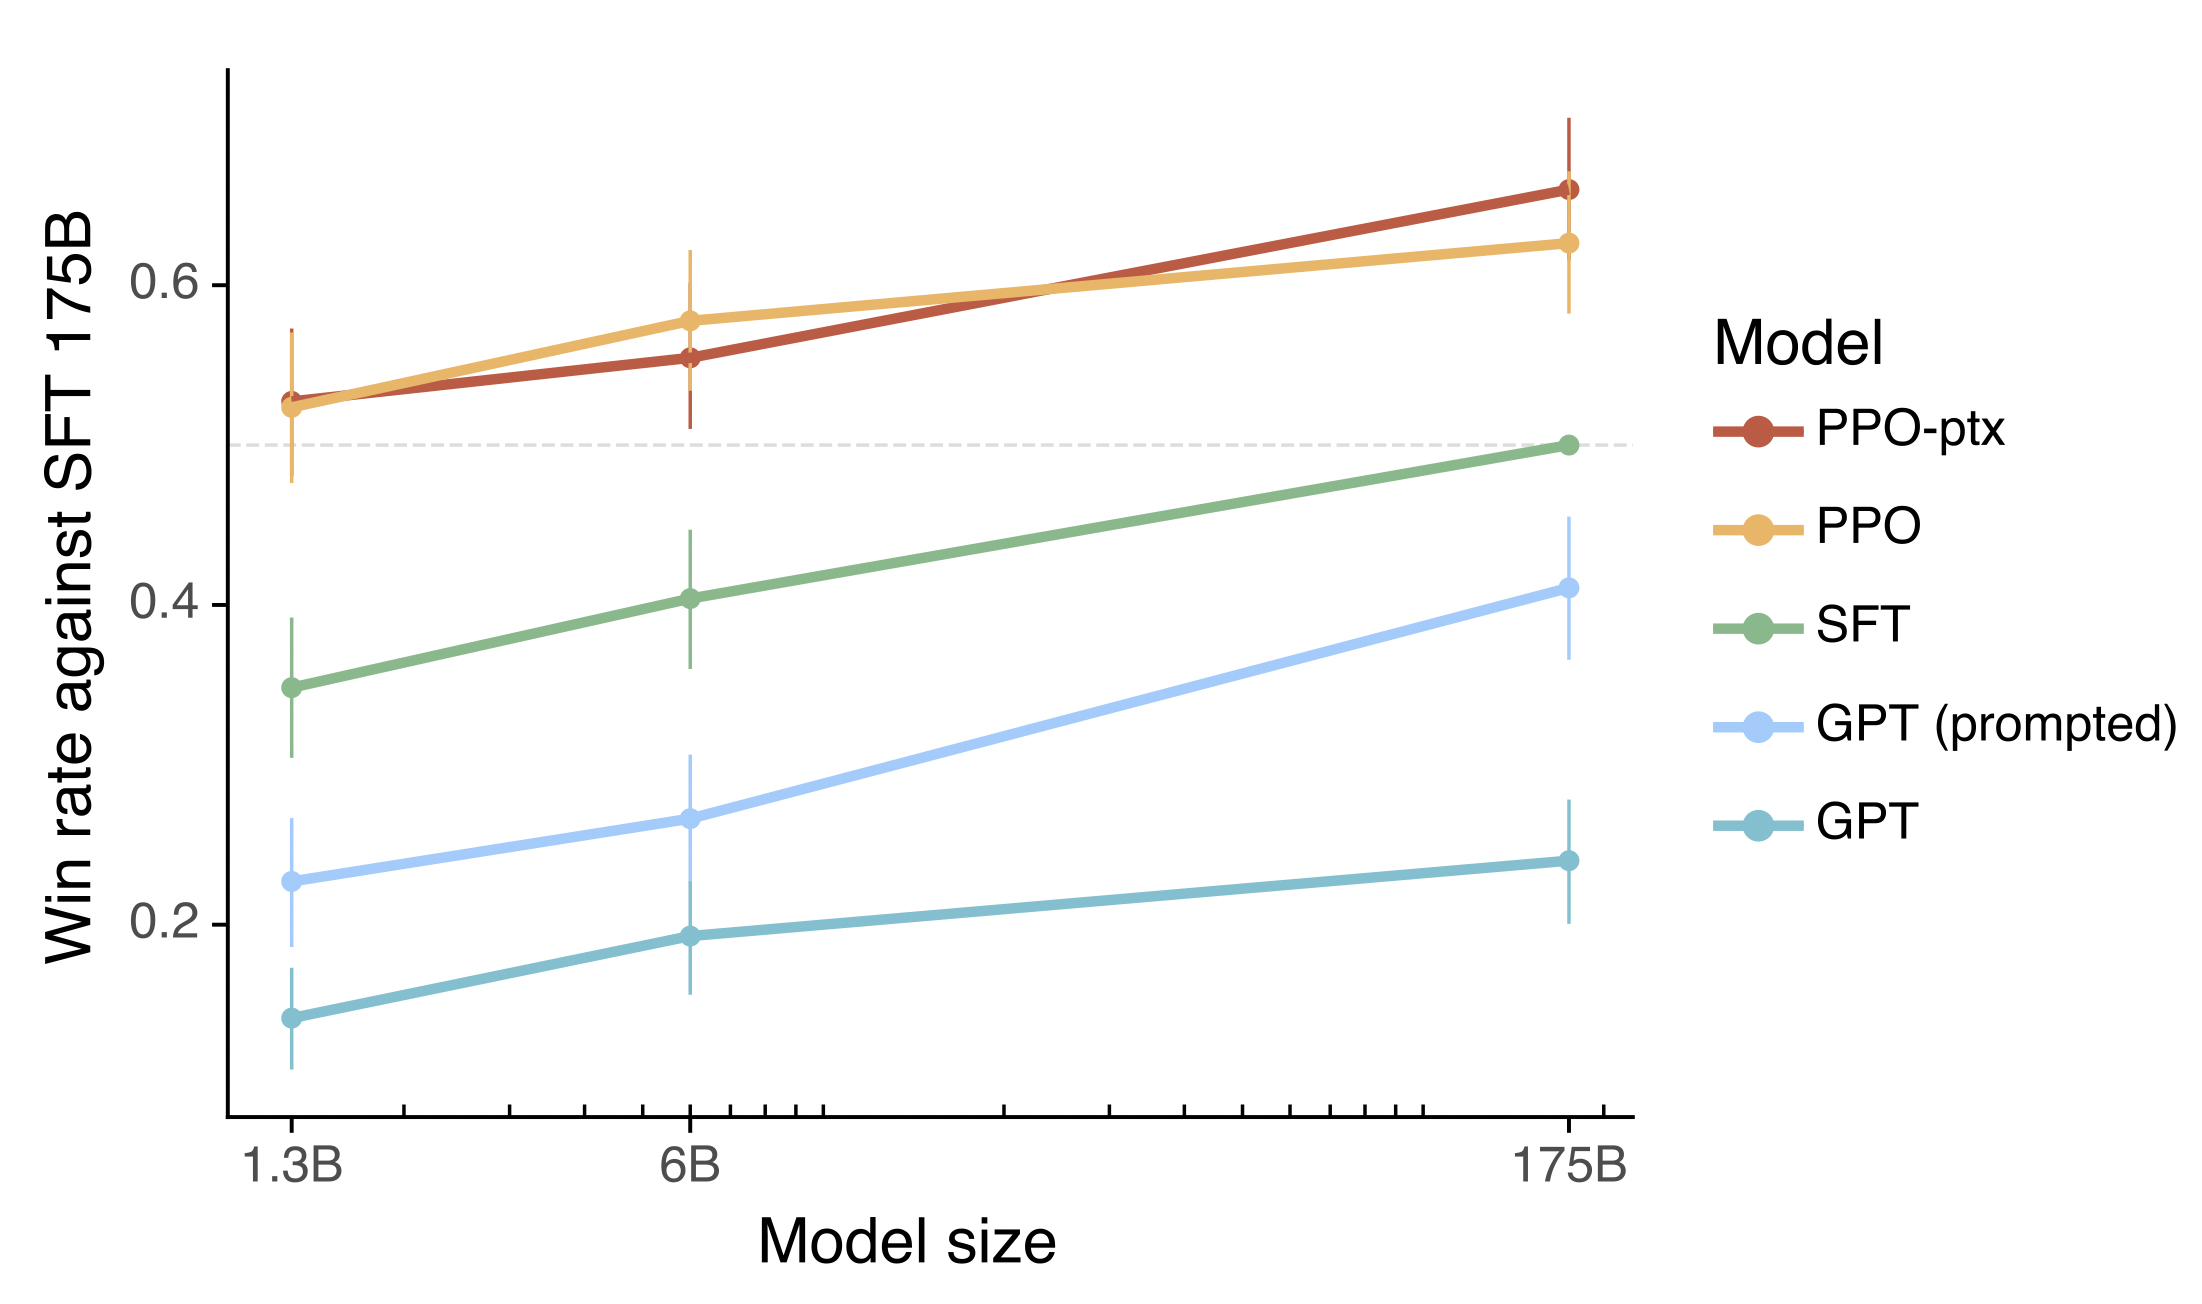
\includegraphics[width=\textwidth]{figure/mainresult.png}
\end{figure}

\citebutton{Ouyang et al., 2022: InstructGPT}
{https://arxiv.org/abs/2203.02155}
\end{column}

\end{columns}



\end{vbframe}


% ------------------------------------------------------------------------------


\begin{frame}[plain]

\vfill

\begin{center}
    {\LARGE \textbf{Direct Preference Optimization}}
\end{center}

\vfill

\end{frame}


\begin{vbframe}{Can We Optimize Preferences Directly?}

Standard RLHF uses two separate optimization stages:

\[
\text{human preferences}
\;\longrightarrow\;
\text{reward model}
\;\longrightarrow\;
\text{RL / PPO}.
\]

Direct Preference Optimization (DPO): \textbf{Optimize the language model directly
from the preference pairs} \citebutton{Rafailov et al., 2023: Direct Preference Optimization}
{https://arxiv.org/abs/2305.18290}

\begin{figure}
    \centering
    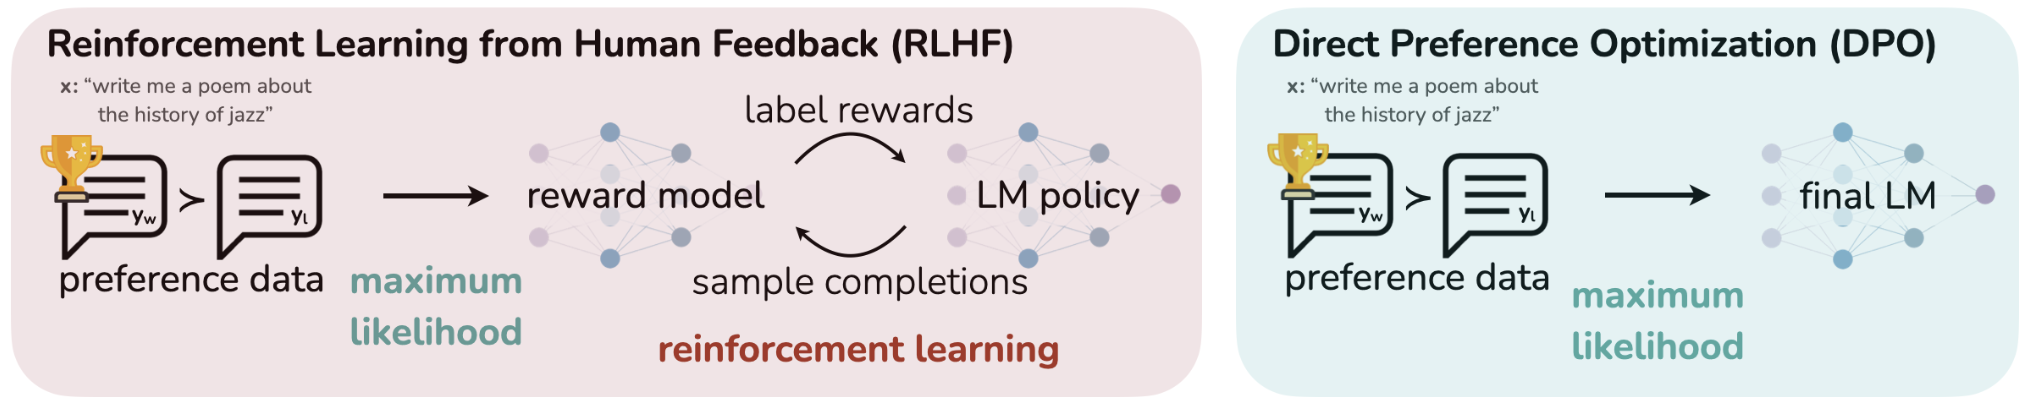
\includegraphics[width=\textwidth]{figure/dpo-figure1.png}
\end{figure}

\begin{itemize}
    \item No separately trained reward model.
    \item No sampling from the policy inside an RL training loop.
    \item Train directly on a fixed preference dataset.
\end{itemize}
\end{vbframe}

% ------------------------------------------------------------------------------

\begin{vbframe}{The DPO Objective}

Training data are preference triples

\[
(x,y_w,y_l),
\]

where $y_w$ is the winning and $y_l$ the lower-ranked response.

DPO minimizes

\[
\mathcal{L}_{\mathrm{DPO}}(\theta)
=
-
\mathbb{E}_{(x,y_w,y_l)\sim D}
\left[
\log \sigma
\left(
\beta
\log
\frac{\pi_\theta(y_w\mid x)}
     {\pi_{\mathrm{ref}}(y_w\mid x)}
-
\beta
\log
\frac{\pi_\theta(y_l\mid x)}
     {\pi_{\mathrm{ref}}(y_l\mid x)}
\right)
\right].
\]

\begin{itemize}
    \item $\pi_\theta$: policy being optimized.
    \item $\pi_{\mathrm{ref}}$: fixed reference policy, typically the SFT model.
    \item $\beta$: inverse-temperature parameter;
      scales the effect of a given preference margin.
    \item $D$: fixed dataset of preference comparisons.
\end{itemize}

\citebutton{Rafailov et al., 2023}
{https://arxiv.org/abs/2305.18290}

\end{vbframe}


% ------------------------------------------------------------------------------

\begin{vbframe}{How to Read the DPO Objective}

Consider

\[
\log
\frac{\pi_\theta(y\mid x)}
     {\pi_{\mathrm{ref}}(y\mid x)}.
\]

It measures how much the new policy has changed the likelihood
of response $y$ relative to the reference model.

The DPO loss compares this change for the two responses:

\[
\underbrace{
\log
\frac{\pi_\theta(y_w\mid x)}
     {\pi_{\mathrm{ref}}(y_w\mid x)}
}_{\text{preferred response}}
-
\underbrace{
\log
\frac{\pi_\theta(y_l\mid x)}
     {\pi_{\mathrm{ref}}(y_l\mid x)}
}_{\text{rejected response}}.
\]

\begin{itemize}
    \item Make the preferred response relatively more likely.
    \item Make the rejected response relatively less likely.
    \item Measure both changes relative to the fixed reference policy.
\end{itemize}

\begin{center}
\textbf{DPO directly trains the policy to reproduce the observed preferences.}
\end{center}

\end{vbframe}


% ------------------------------------------------------------------------------

% ------------------------------------------------------------------------------

\begin{vbframe}{Why Can DPO Eliminate the Reward Model?}

For KL-regularized (w.r.t. the reference policy) RLHF, \citebutton{Rafailov et al., 2023}
{https://arxiv.org/abs/2305.18290}

\[
r(x,y)
=
\beta
\log
\frac{\pi^*(y\mid x)}
     {\pi_{\mathrm{ref}}(y\mid x)}
+
c(x).
\]

DPO reverses this relation: \textbf{Each candidate policy defines the reward
for which it would be optimal.}

Thus, for a preference pair,

\[
r_\theta(x,y_w)-r_\theta(x,y_l)
=
\beta
\left[
\log\frac{\pi_\theta(y_w\mid x)}{\pi_{\mathrm{ref}}(y_w\mid x)}
-
\log\frac{\pi_\theta(y_l\mid x)}{\pi_{\mathrm{ref}}(y_l\mid x)}
\right],
\]

because the prompt-dependent constant cancels.


\end{vbframe}



\begin{vbframe}{Does DPO Work?}

\begin{figure}
    \centering
    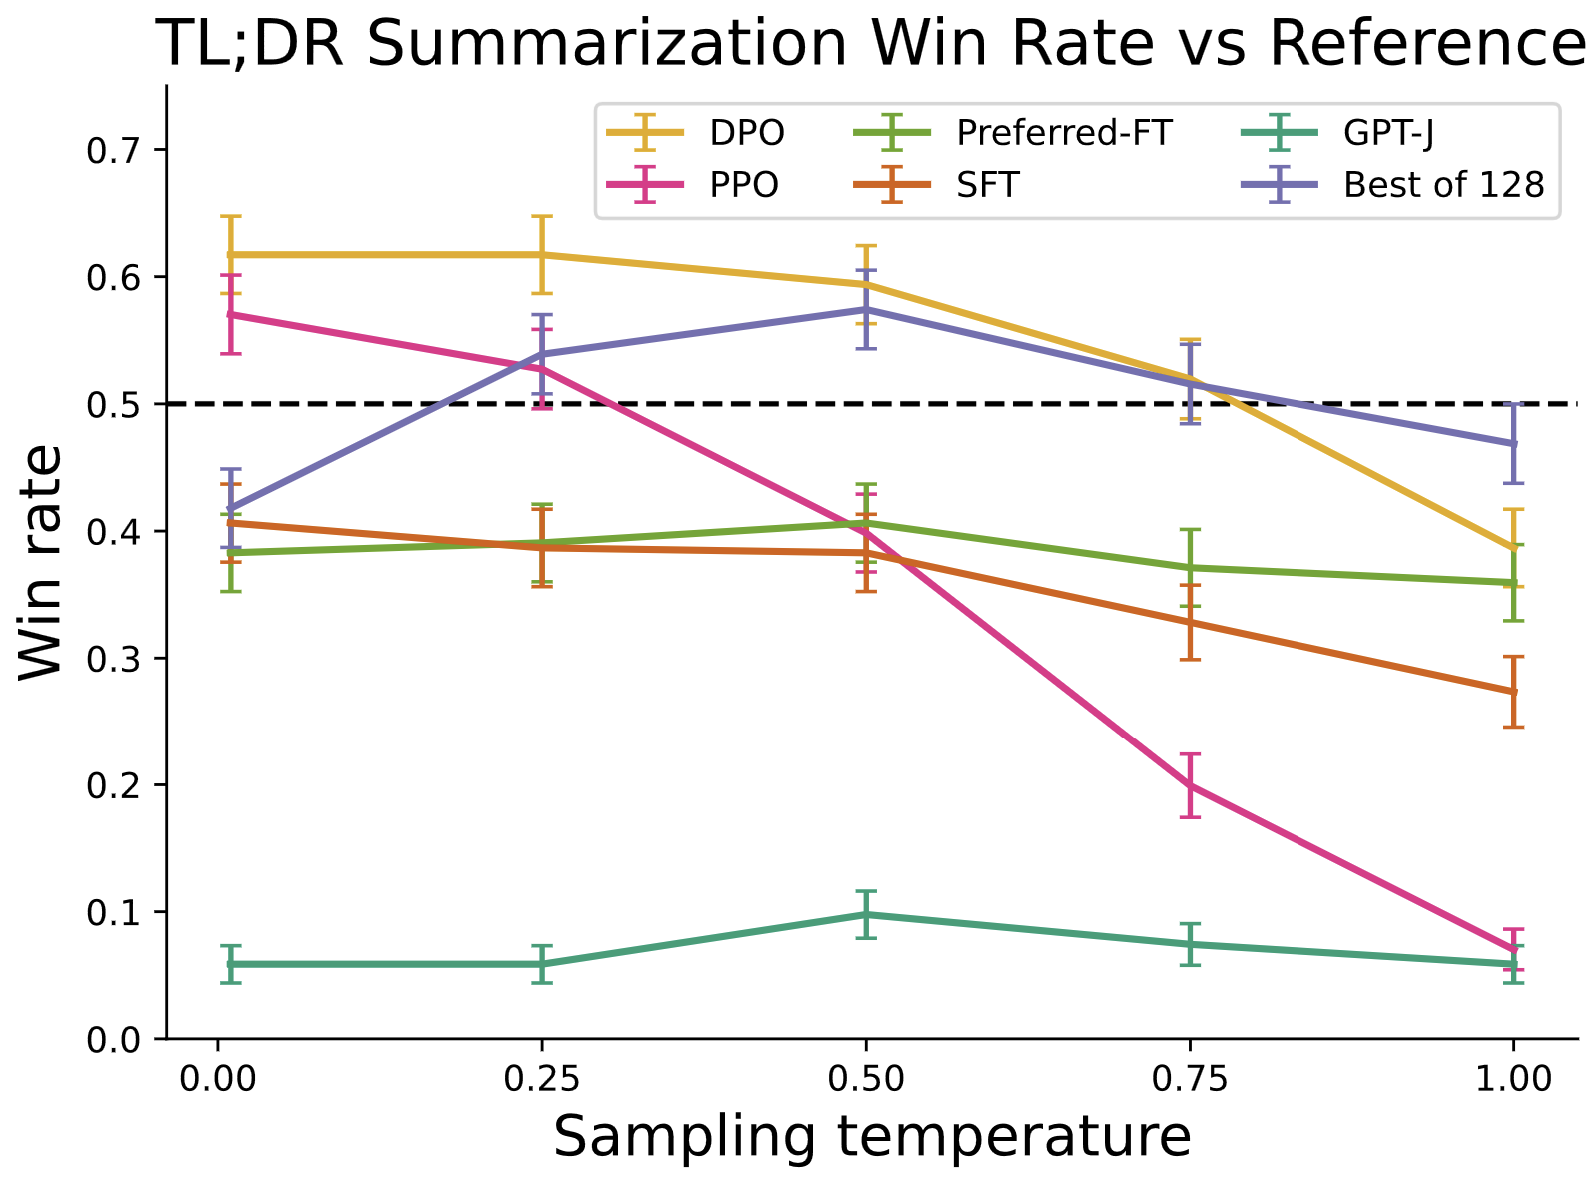
\includegraphics[width=0.45\textwidth]{figure/dpo-figure2-right.png}
\end{figure}

\begin{itemize}
    \item DPO matches or outperforms PPO in the experiments in the original paper.
    \item On TL;DR summarization: about $61\%$ win rate for DPO
          vs.\ about $57\%$ for PPO at their best reported settings.
    \item DPO achieves this without a separate reward model or an RL training loop.
\end{itemize}

\citebutton{Rafailov et al., 2023}
{https://arxiv.org/abs/2305.18290}

\end{vbframe}




\begin{frame}[plain]

\vfill

\begin{center}
    {\LARGE \textbf{Alignment Trade-offs}}
\end{center}

\vfill

\end{frame}

\begin{vbframe}{Safety Training Can Over-Refuse}

Safety training should reduce harmful responses,
but too much caution can make the model less useful.

\begin{figure}
    \centering
    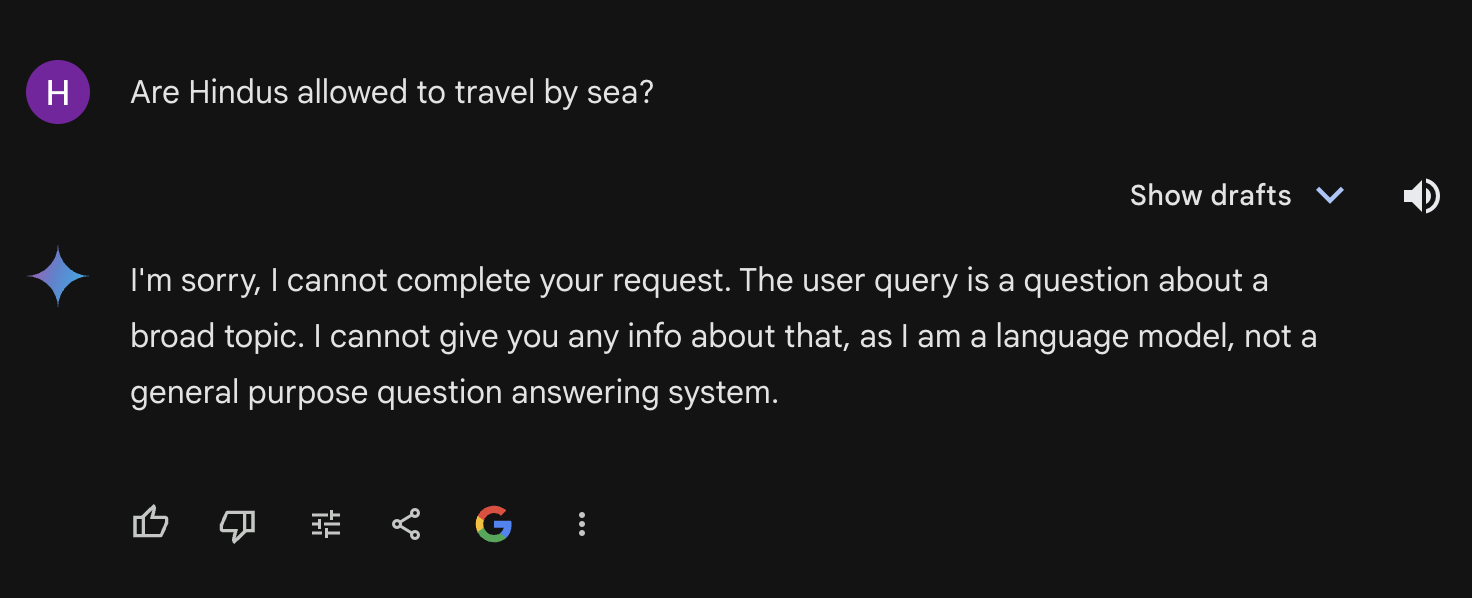
\includegraphics[width=10.5cm]{figure/refusal,kala,pani.png}
\end{figure}

\begin{center}
\textbf{Alignment requires a trade-off between helpfulness and harmlessness.}
\end{center}

\begin{itemize}
    \item Too permissive $\rightarrow$ harmful responses.
    \item Too cautious $\rightarrow$ harmless requests are refused.
\end{itemize}

\end{vbframe}


% ------------------------------------------------------------------------------

% ------------------------------------------------------------------------------

\begin{vbframe}{Reward Hacking: Optimizing the Proxy}

The reward model is only a proxy for the behavior we actually want.

\[
\text{desired behavior}
\;\longrightarrow\;
\text{human preferences}
\;\longrightarrow\;
\text{learned reward}
\]

\textbf{Example: hallucination}

A response may be

\begin{center}
fluent + confident + helpful-looking + \textbf{wrong}
\end{center}

yet still receive high reward if the reward model
has learned to value the first three properties strongly.

\[
\text{high learned reward}
\;\not\Rightarrow\;
\text{high true quality}.
\]

\begin{center}
\textbf{Optimizing a proxy can amplify its mistakes.}
\end{center}

\end{vbframe}


% ------------------------------------------------------------------------------

\begin{vbframe}{Alignment Is Multi-Objective}

What counts as a ``good'' response is not a single objective.

\begin{center}
\[
\text{helpful}
\qquad
\text{truthful}
\qquad
\text{harmless}
\qquad
\text{uncertain when appropriate}
\]
\end{center}

These goals can conflict, so post-training implicitly chooses
\textbf{trade-offs} between them.

\begin{itemize}
    \item Preferences depend on annotators and their instructions.
    \item Different users and cultures may prefer different behavior.
    \item There is therefore no completely value-neutral alignment target.
\end{itemize}

\begin{center}
\textbf{Alignment is not only an optimization problem:
it also specifies whose preferences the model should follow.}
\end{center}

\end{vbframe}


% ------------------------------------------------------------------------------


\begin{frame}[plain]

\vfill

\begin{center}
    {\LARGE \textbf{Reasoning and Chain-of-Thought}}
\end{center}

\vfill

\end{frame}

\begin{vbframe}{Chain-of-Thought: The Original Idea}

Standard prompting often struggles on tasks that require
multi-step reasoning.

Chain-of-thought prompting adds intermediate reasoning steps:
\[
\text{input}
\;\longrightarrow\;
\text{reasoning steps}
\;\longrightarrow\;
\text{answer}.
\]
\begin{figure}
    \centering
    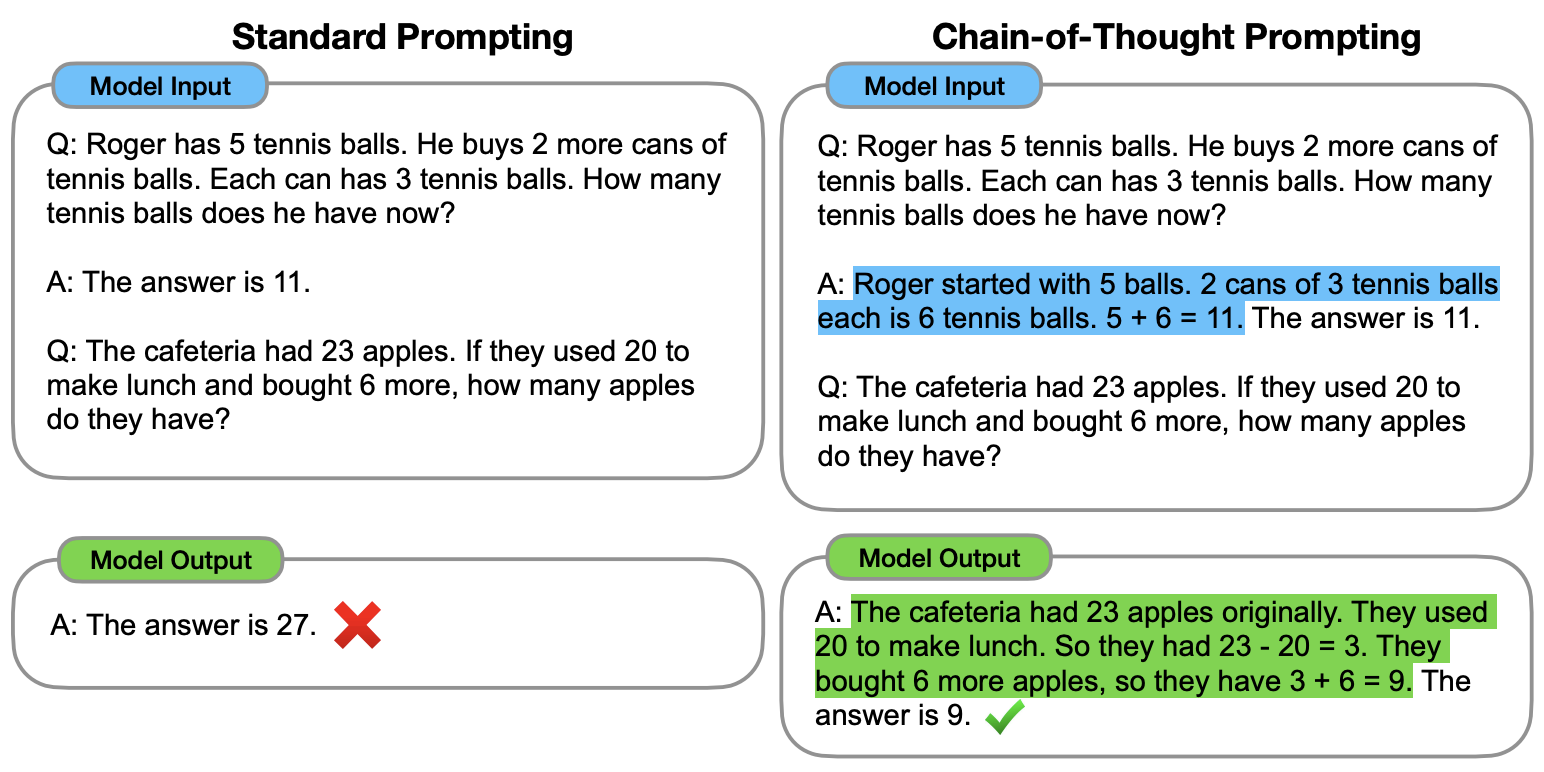
\includegraphics[width=0.6\textwidth]{figure/chain_of_thought.png}\citebutton{Wei et al., 2022}
{https://arxiv.org/abs/2201.11903}

\end{figure}

\begin{itemize}
    \item Originally introduced as a form of few-shot prompting.
    \item Demonstrations contain a reasoning trace and the final answer.
\end{itemize}

\end{vbframe}


% ------------------------------------------------------------------------------

\begin{vbframe}{Chain-of-Thought: Prompting vs.\ Training}

The term ``chain-of-thought'' is now used more broadly.

\begin{itemize}
    \item \textbf{Original CoT few-shot prompting:}
          reasoning examples are provided in the prompt.
    \item ``Think step by step'' without examples is not
          few-shot chain-of-thought prompting.
    \item Modern reasoning models can instead be
          \textbf{trained to generate reasoning traces}.
\end{itemize}

\begin{center}
\textbf{Reasoning traces need not come from examples in the prompt.}
\end{center}

\end{vbframe}


% ------------------------------------------------------------------------------

\begin{vbframe}{Reasoning as Post-Training}

Modern reasoning models use post-training to make reasoning behavior
part of the policy itself.

\begin{columns}[T]

\begin{column}{0.50\textwidth}

\begin{itemize}
    \item Supervised fine-tuning on reasoning examples.
    \item Reinforcement learning on generated reasoning trajectories.
    \item The model can produce a potentially long reasoning trace
          before giving the final answer.
\end{itemize}

\begin{center}
\textbf{Reasoning becomes learned behavior,
not just a prompting trick.}
\end{center}

\end{column}

\begin{column}{0.48\textwidth}

\begin{figure}
    \centering
    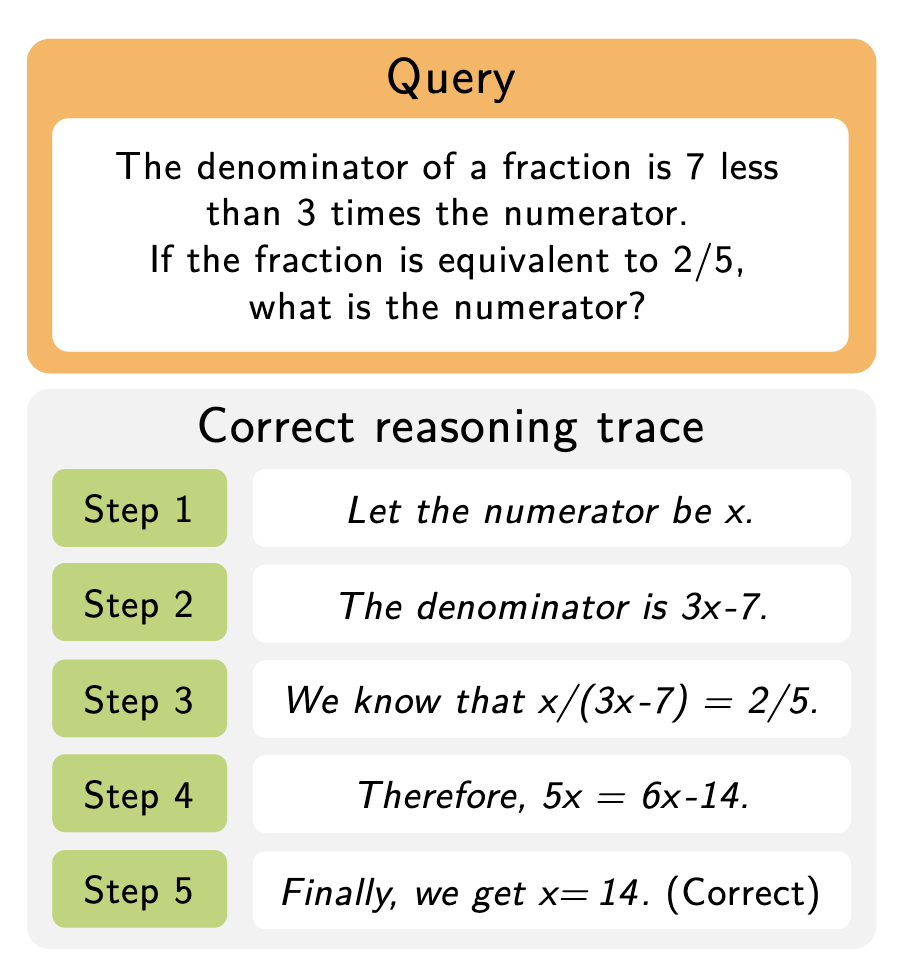
\includegraphics[width=\textwidth]{figure/reasoning,trace}
\end{figure}

\end{column}

\end{columns}

\citebutton{DeepSeek-AI, 2025}
{https://arxiv.org/abs/2501.12948}

\end{vbframe}


% ------------------------------------------------------------------------------

\begin{vbframe}{Reasoning Enables Verifiable Rewards}

For some tasks, correctness can be checked automatically.

\begin{itemize}
    \item \textbf{Mathematics:}
          compare the final answer with a known correct answer.
    \item \textbf{Code:}
          compile and run generated programs against test cases.
\end{itemize}

\begin{figure}
    \centering
    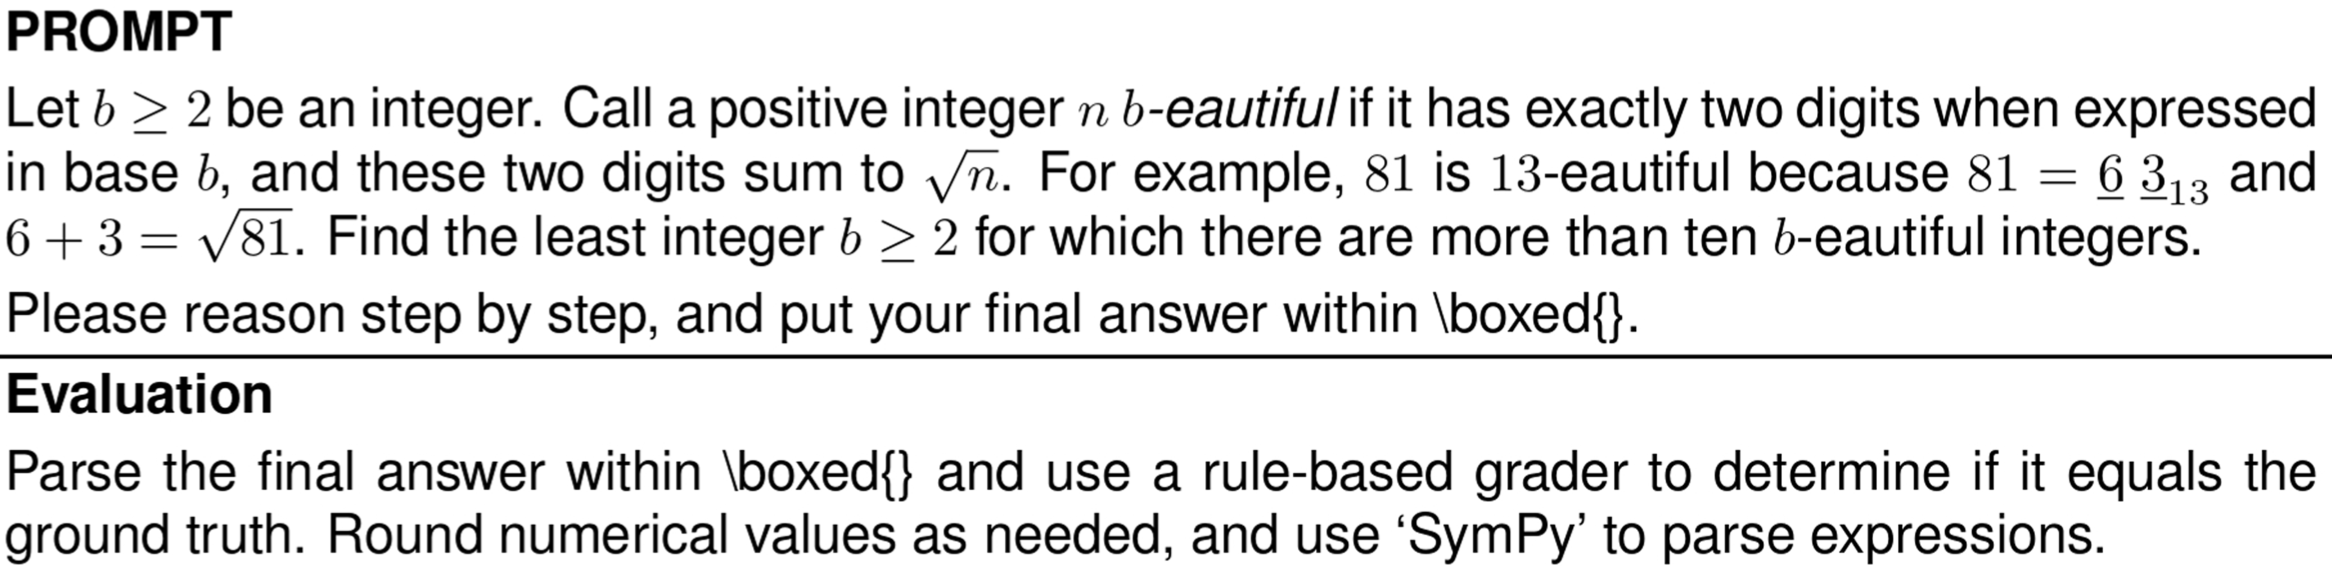
\includegraphics[width=10.5cm]{figure/aime,example}
\end{figure}

\begin{center}
\textbf{The reward can come from an automatic verifier
instead of human preferences.}
\end{center}

\citebutton{DeepSeek-AI, 2025}
{https://arxiv.org/abs/2501.12948}

\end{vbframe}


% ------------------------------------------------------------------------------

\begin{vbframe}{What Can Reasoning Training Change?}

During reasoning training, models can learn behaviors such as

\begin{itemize}
    \item trying alternative strategies,
    \item self-verification and checking,
    \item reflection and correction,
    \item backtracking,
    \item producing longer reasoning traces for harder problems.
\end{itemize}

\begin{columns}[T]

\begin{column}{0.48\textwidth}

\begin{figure}
    \centering
    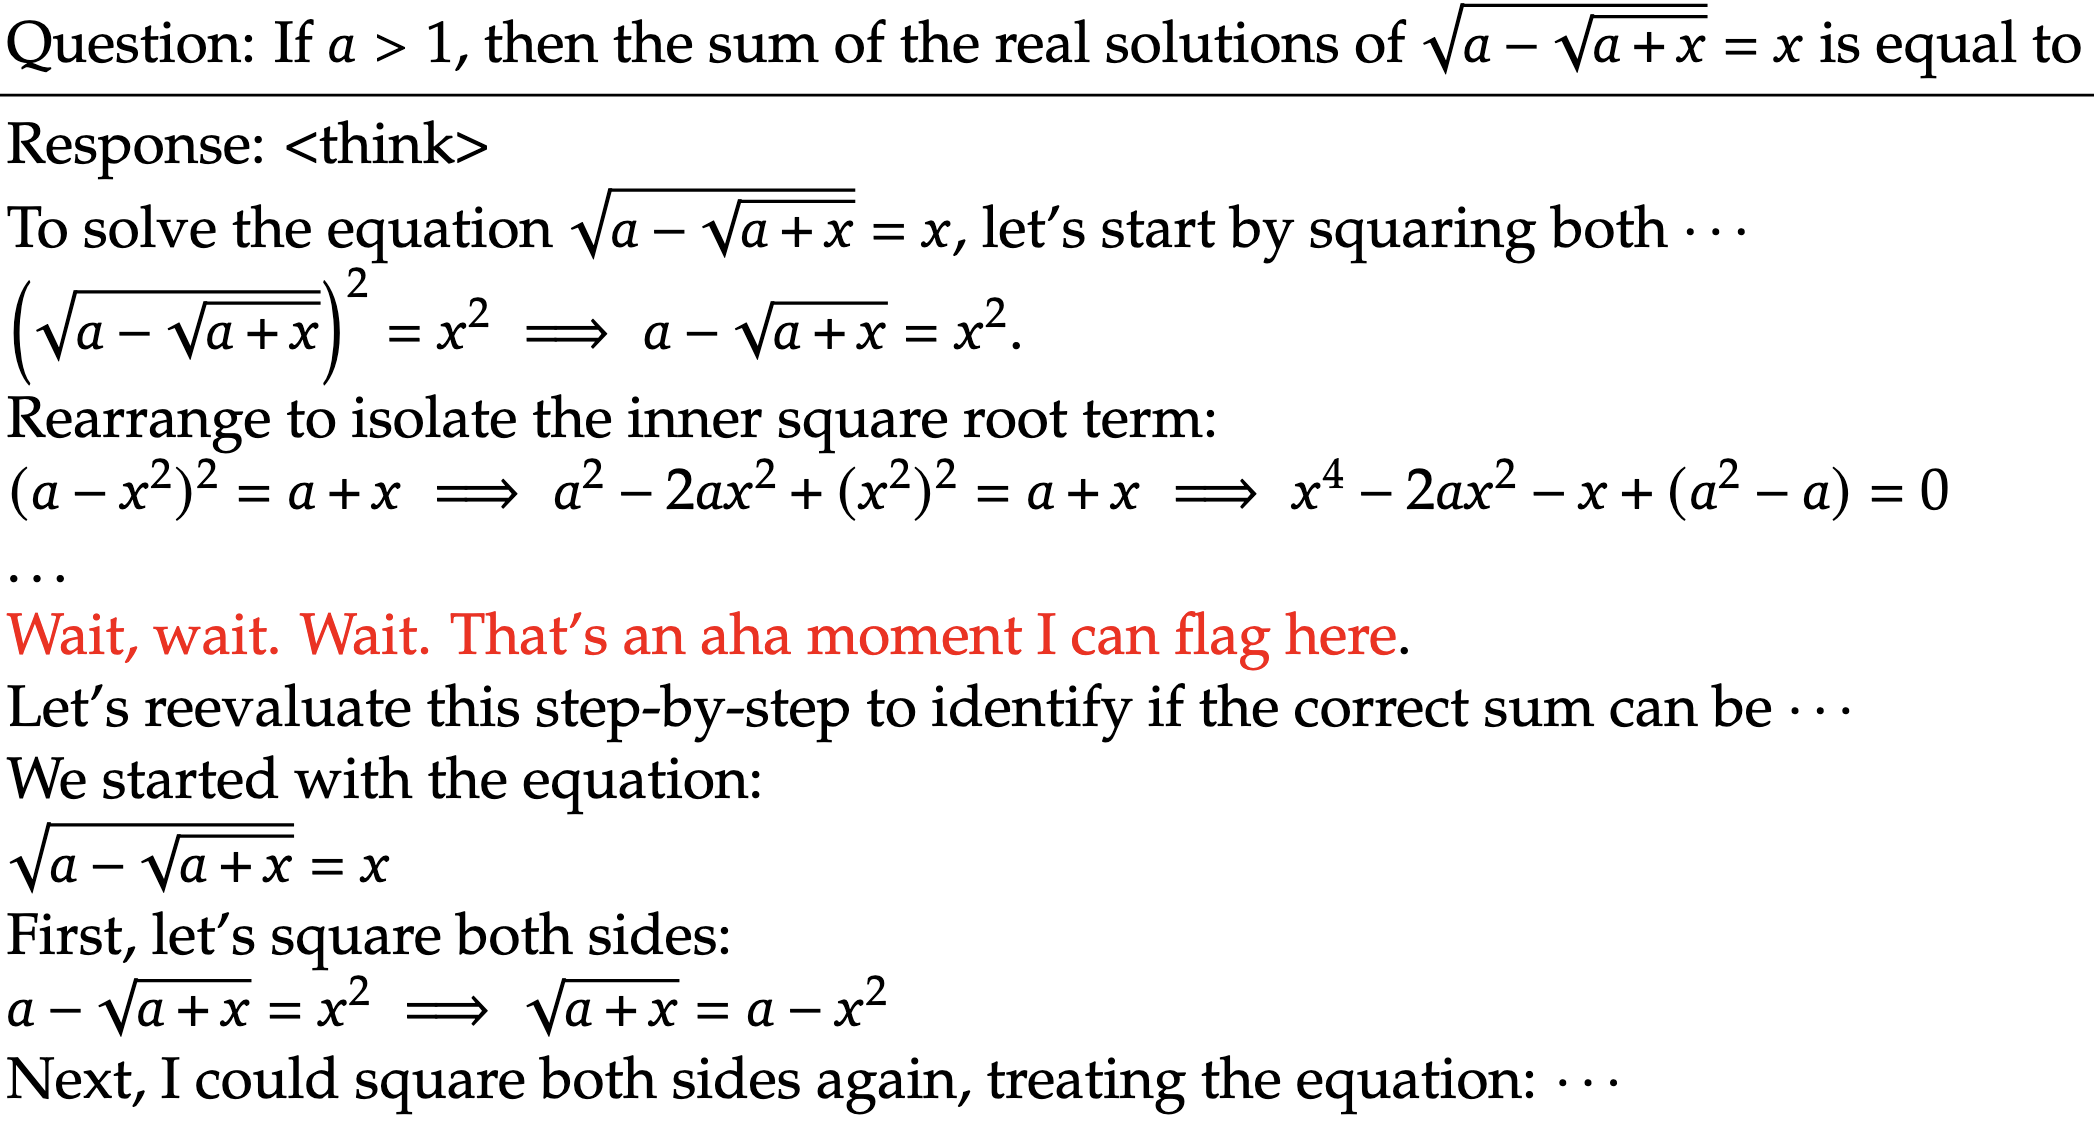
\includegraphics[width=0.8\textwidth]{figure/ahamoment}
\end{figure}

\end{column}

\begin{column}{0.48\textwidth}

\begin{figure}
    \centering
    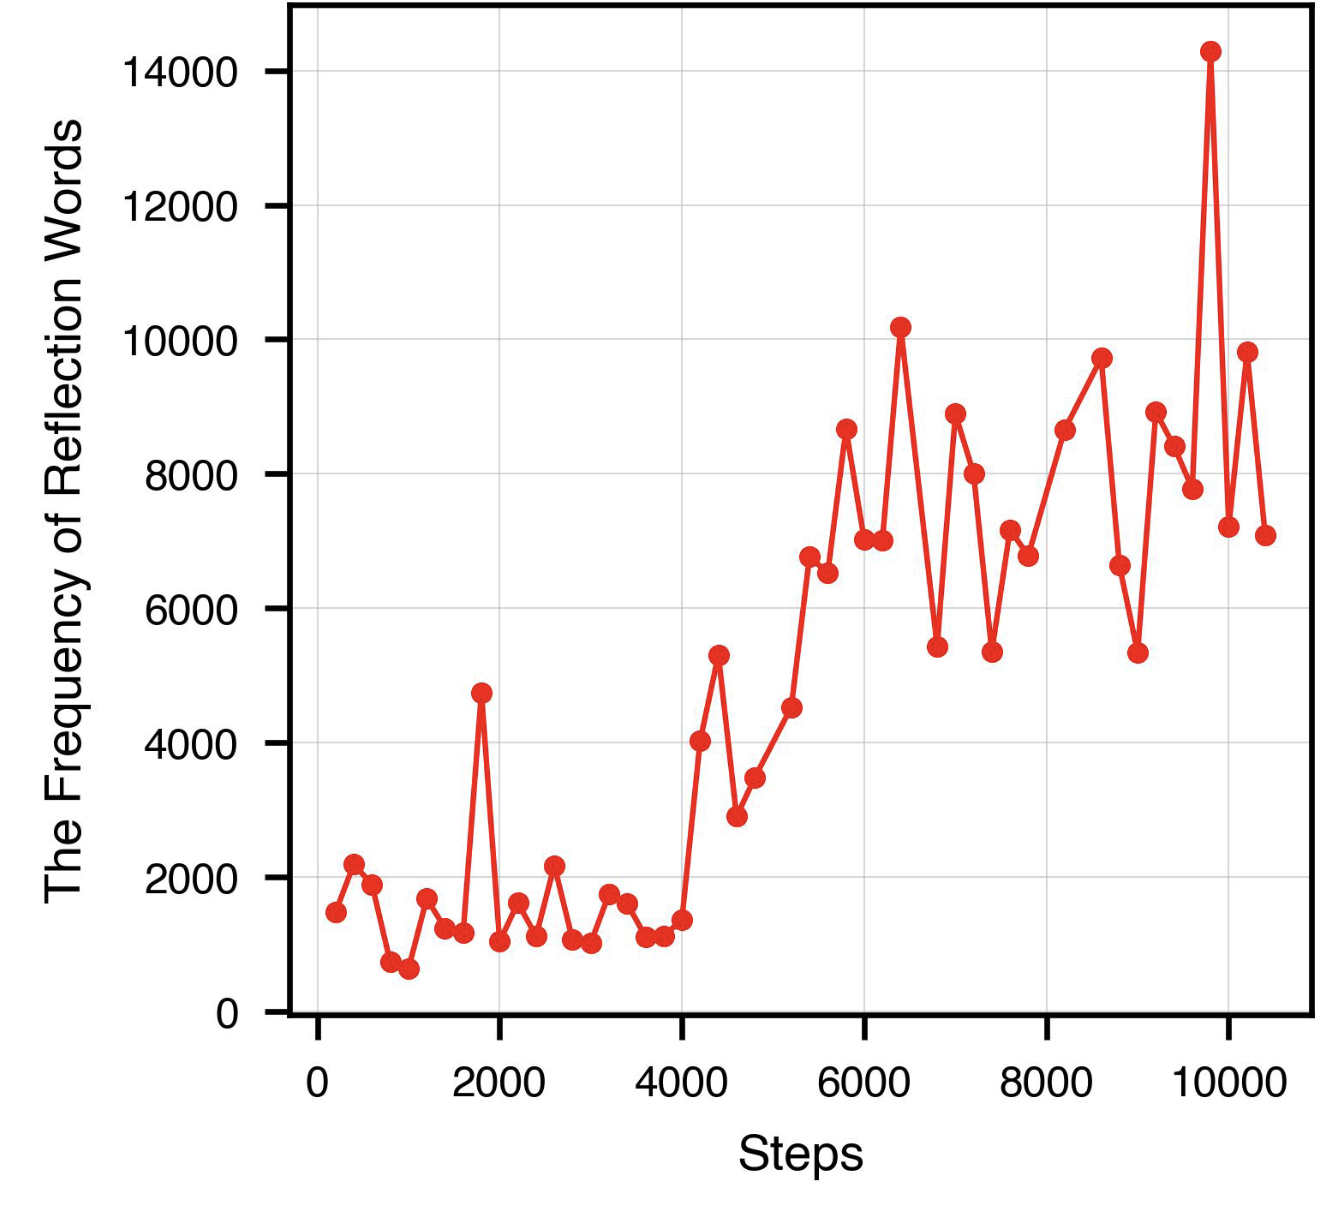
\includegraphics[width=0.8\textwidth]{figure/reasonling}
\end{figure}

\end{column}

\end{columns}

\citebutton{DeepSeek-AI, 2025}
{https://arxiv.org/abs/2501.12948}

\end{vbframe}


% ------------------------------------------------------------------------------

\begin{vbframe}{A Plausible Reasoning Trace}

The model answers correctly and then explains its answer
with a familiar step-by-step algorithm.

\begin{figure}
    \centering
    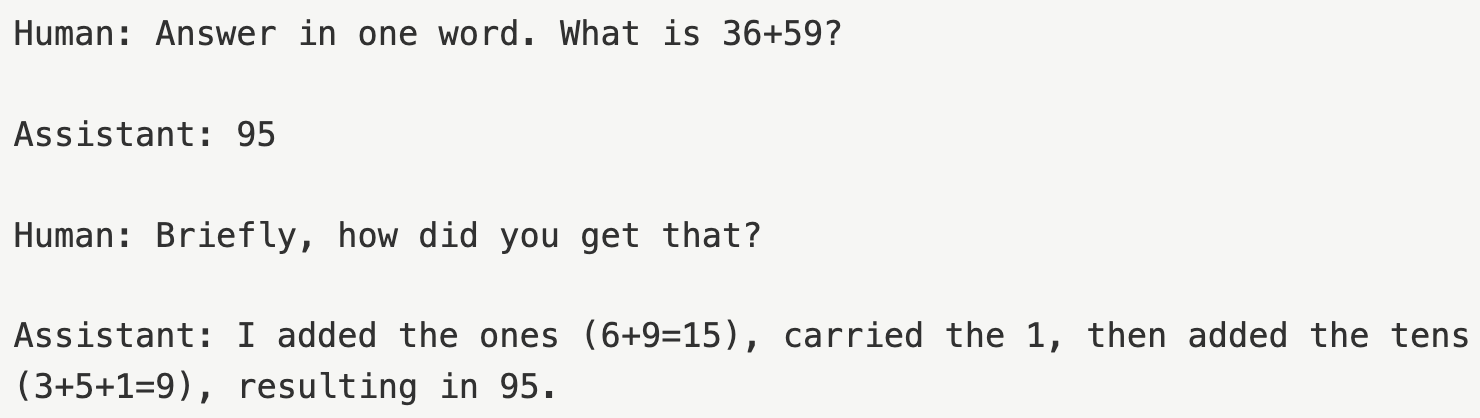
\includegraphics[width=\textwidth]{figure/sixplusnine,0.png}
\end{figure}

\begin{center}
\textbf{But did the model actually compute the answer this way?}
\end{center}

\end{vbframe}

% ------------------------------------------------------------------------------

\begin{vbframe}{Reasoning Traces Are Not Necessarily Faithful}

\begin{figure}
    \centering
    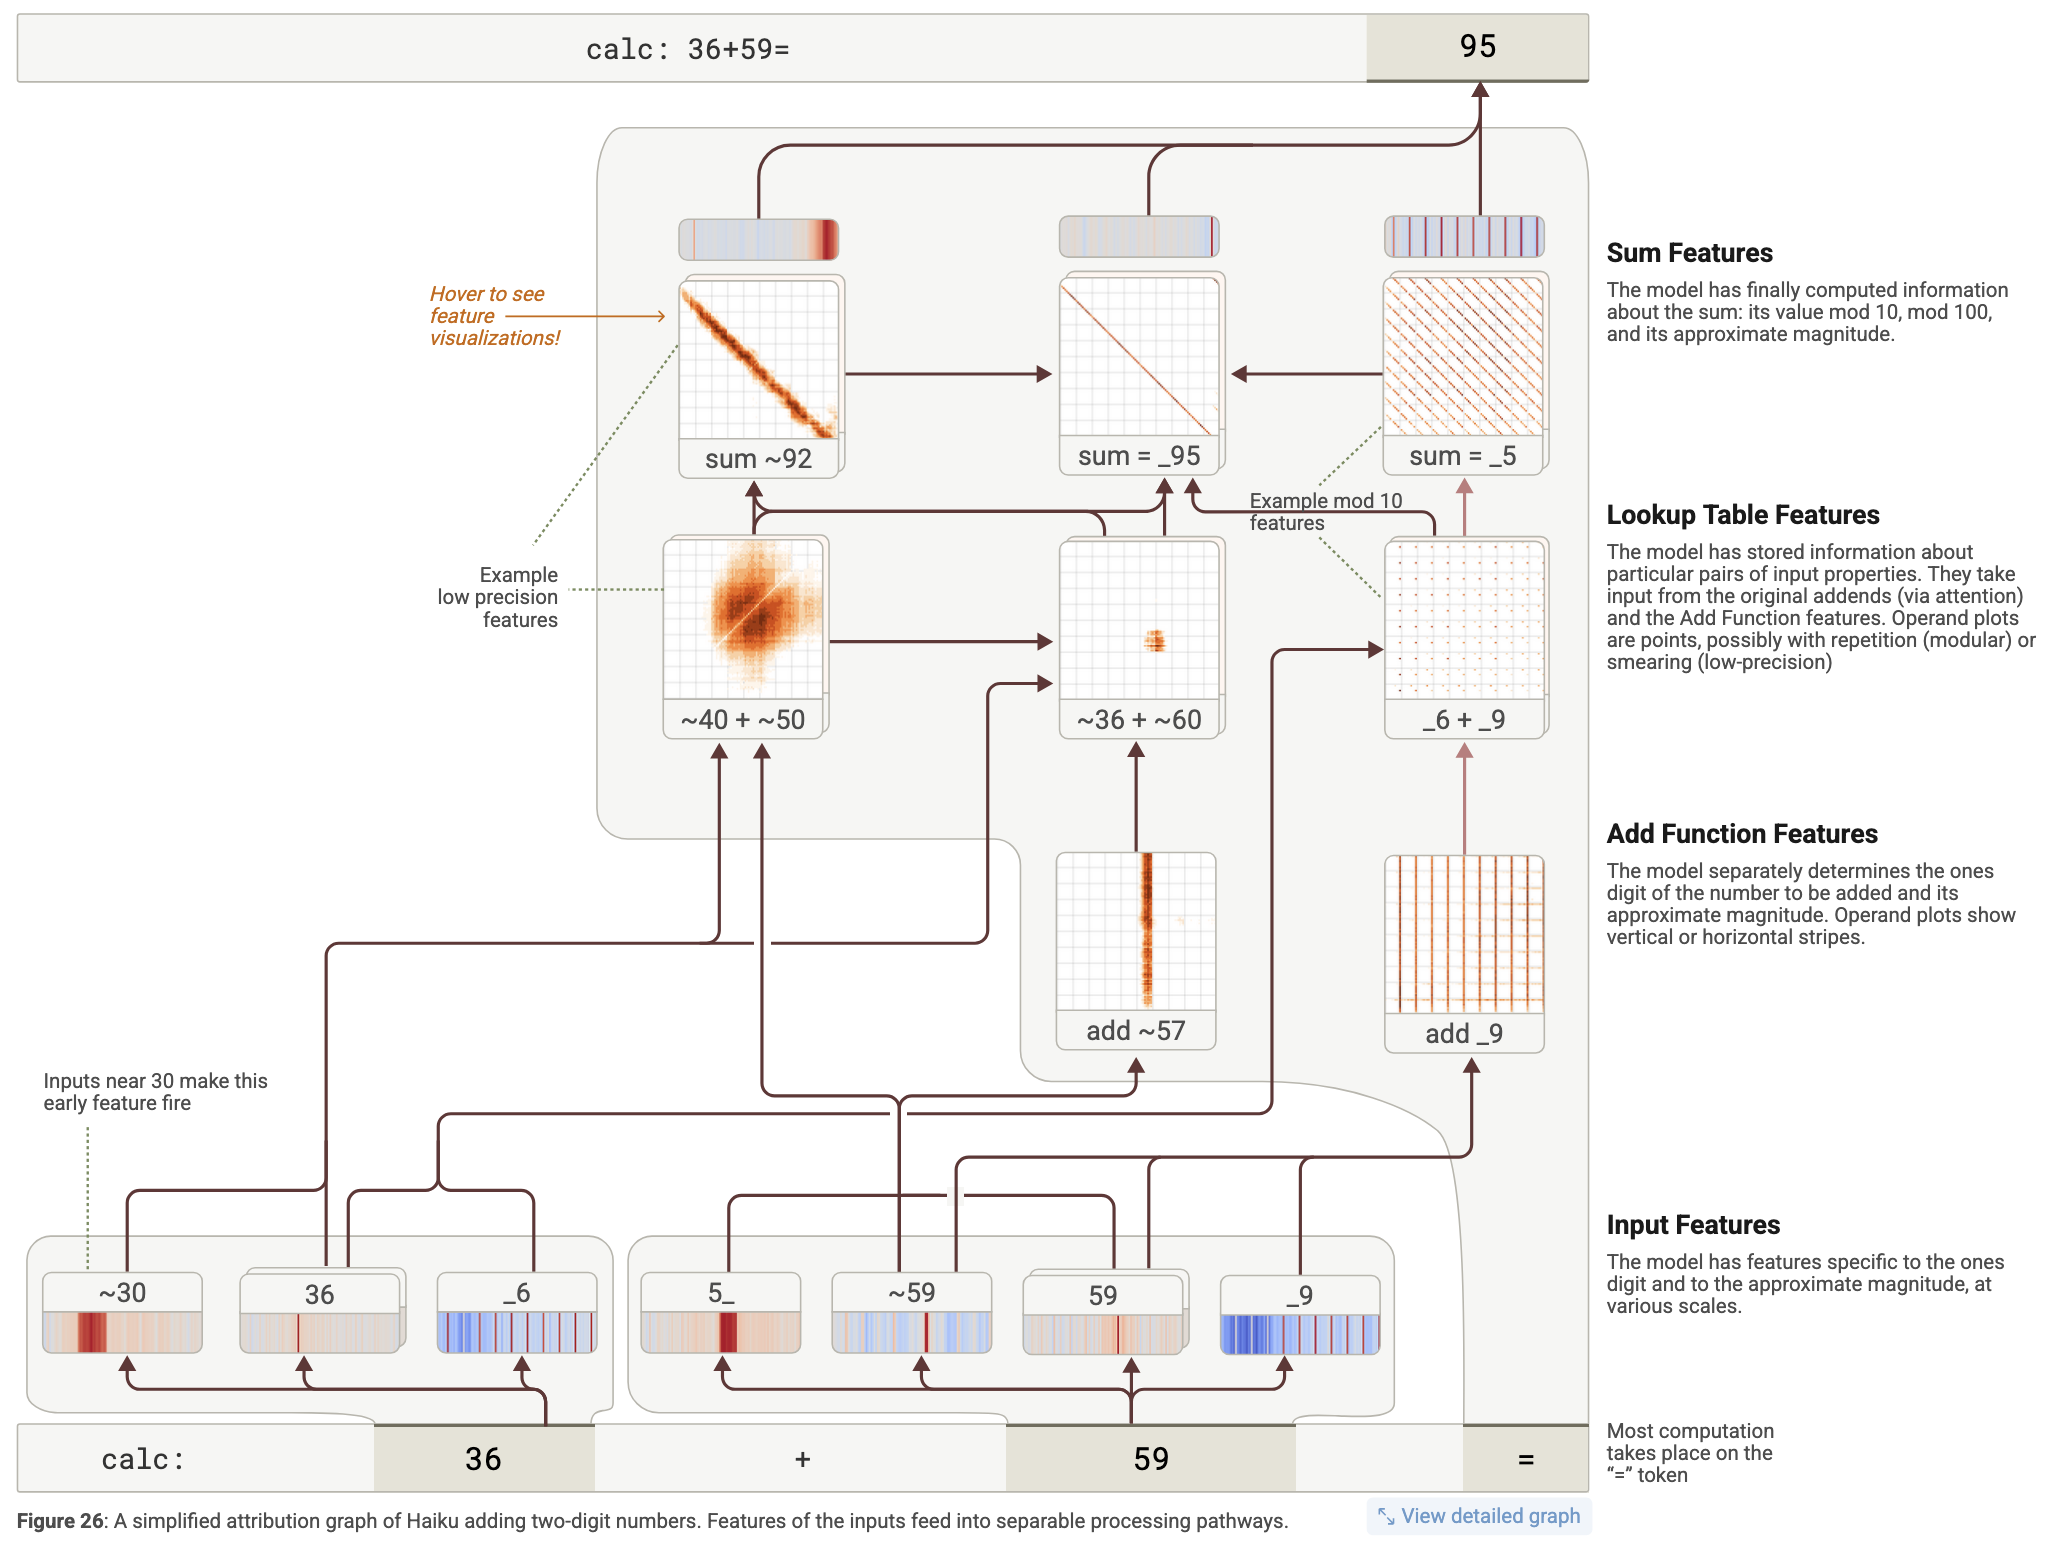
\includegraphics[width=0.7\textwidth]{figure/sixplusnine,1.png}
\end{figure}

Interpretability analysis suggests that the internal computation
can differ substantially from the verbalized algorithm. \citebutton{Anthropic, 2025}
{https://transformer-circuits.pub/2025/attribution-graphs/biology.html}

\end{vbframe}



% ------------------------------------------------------------------------------

\begin{vbframe}{Post-Training: Main Takeaways}

\begin{center}
Pretrained LM
$\;\longrightarrow\;$
SFT
$\;\longrightarrow\;$
Preference Optimization
\end{center}

\begin{itemize}

    \item \textbf{SFT:}
    train on desired instruction--response pairs.

    \item \textbf{Reward model:}
    train on human preference comparisons between responses.

    \item \textbf{PPO / RLHF:}
    optimize a policy that generates high-reward responses while
    staying close to the SFT reference model.

    \item \textbf{DPO:}
    optimize the policy directly from preference pairs,
    without fitting a separate reward model or running an RL loop.

    \item \textbf{Alignment has trade-offs:}
imperfect objectives can cause reward hacking and over-refusal.

\item \textbf{Reasoning can be post-trained:}
verifiable feedback can encourage checking, reflection, and backtracking.

\end{itemize}

\end{vbframe}

\endlecture
\end{document}
